\documentclass[article]{report}         % Type of document

\usepackage[utf8]{inputenc}             % Encoding
\usepackage[english]{babel}             % Language
\usepackage{geometry}                   % Page margin
\usepackage{graphicx}                   % For images
\usepackage{newcent}                    % Font
\usepackage{color}                      % Colors
\usepackage{listings}                   % Lists
\usepackage[footnote, nolist]{acronym}  % Acronyms
\usepackage[absolute, overlay]{textpos} % Text positioning
\usepackage[babel=true]{csquotes}

\usepackage{fancyhdr}
\usepackage{float}
\usepackage{tabularx}

\usepackage{latexsym}
\usepackage{pdfpages}
\usepackage{tikz}
\usepackage{ifthen}
\usepackage{wrapfig}
\usepackage{textcomp}
\usepackage{multicol}

\usepackage{listings} % includes code

\lstset{
  tabsize=4,
  language=matlab,
        basicstyle=\scriptsize,
        %upquote=true,
        aboveskip={0.5\baselineskip},
        columns=fixed,
        showstringspaces=false,
        extendedchars=true,
        breaklines=true,
        basicstyle=\normalsize,
        prebreak = \raisebox{2ex}[2ex][2ex]{\ensuremath{\hookleftarrow}},
        showtabs=false,
        showspaces=false,
        showstringspaces=false,
        identifierstyle=\ttfamily,
        keywordstyle=\color[rgb]{0,0,1},
        commentstyle=\color[rgb]{0.133,0.545,0.133},
        stringstyle=\color[rgb]{0.627,0.126,0.941},
  language=Java
}

\setlength{\columnsep}{1cm}
\setlength{\TPHorizModule}{\paperwidth} % Used for textblock
\setlength{\TPVertModule}{\paperheight} % Used for textblock
\parskip = 0.25cm              % Summary options (spaces between lines)

% Margin
\geometry{tmargin=2.5cm, bmargin=1.5cm, lmargin=2.5cm, rmargin=2cm}

\definecolor{blue}{rgb}{0.13,0.29,0.46}
\definecolor{red}{rgb}{1,0,0}
\definecolor{couleur_titre}{rgb}{0.20, 0.45, 0.80}
\definecolor{couleur_nom}{rgb}{0.11, 0.6, 0.18}

\renewcommand{\labelitemi}{$\bullet$}
\renewcommand{\contentsname}{Table of contents}

% Title at the top of the page
\pagestyle{fancyplain} \chead{}\lhead{\textit{Team Dedalus}} \rhead{\textcolor{couleur_titre}{\emph{\textit{Project: SkyLands}}}}

\title {Oral presentation 4}
\author {Romain\and Renaud\and Aenora\and Erwan}
\date {}

%
% Document
%
\begin{document}
  \thispagestyle{empty}
    \begin{titlepage} 
    \vspace*{1cm} 
      \begin{center} 
        {\huge{\textsc{4th Oral Presentation} \\ ~ \\{\large From}\\ ~\\ Team \\  ~ \\ }}
        \includegraphics[width = 14cm]{images/Titles/Dedalus.png}
      \\ ~ \\ ~ \\ ~ \\ ~ \\ ~ \\ ~ \\ ~ \\ ~ \\ ~ \\ ~ \\ ~ \\ ~ \\ ~ \\ ~ 
    \end{center}
      \hfill {\large Erwan  \textsc{Vasseure}}
      \hfill {\large Aenora \textsc{Tye}}
      \hfill {\large Renaud \textsc{Gaubert}}
      \hfill {\large Romain \textsc{Biessy}}
    \end{titlepage} 

    \tableofcontents
      \pagenumbering{arabic}
      \setcounter{page}{2}
      \newpage
    \chapter{\textcolor{blue}{Introduction}}
      Markus ``Notch'' Persson spent two years on Minecraft full time, helped with five to ten people who were all experienced game developers. \\
      As for us, students of Epita, we spent a mere nine month developing and, the result is an awesome game!\\

      SkyLands is a Minecraft-like game in which we added some strategy. Thus you are able to create units and buildings in order to defeat your foes just like a strategy game, except that it's in a Minecraft world!\\

      At Dedalus corporation we like the variety of languages as well as new technologies! Thus our project has been coded using five differente languages and uses about four frameworks.\\
      At first there is our 3d engine Ogre written in C++ then our Game which uses Ogre is mostly written in C\#. But then what's interesting is that we don't have a GUI but a web UI thus we are using not only HTML and CSS in our menus but JavaScript as well!

        \chapter{\textcolor{blue}{Licensing}}
          At Dedalus, we consider that Licensing our code is an important task. According to the French legal code, a license is an authorization.\\
          First, we explored the available licenses and, one of the first license we were directed to was the GNU GPL.

          \section{GNU LGPL}
            \begin{textblock}{0.475}(0.120, 0.470)
              The GNU Lesser General Public License or LGPL (formerly the GNU Library General Public License) is a free software license published by the Free Software Foundation (FSF). \\
              The LGPL allows developers and companies to use and integrate LGPL software into their own (even proprietary) software without being required (by the terms of a strong copyleft) to release the source code of their own software-parts. Merely the LGPL software-parts need to be modifiable by end-users (via source code availability): therefore, in the case of proprietary software, the LGPL-parts are usually used in the form of a shared library (e.g. DLL), so that there is a clear separation between the proprietary parts and open source LGPL parts.\\
          \end{textblock}

          \begin{textblock}{0.628}(0.600, 0.495)
            \begin{figure}
              
\includegraphics[width=6.5cm]{images/LGPL.png}
            \end{figure}
          \end{textblock}
          ~\\~\\~\\~\\~\\~\\~\\~\\~\\~\\~\\~\\~\\
          However one of the downside of the LGPL is that if you do not use the code in a DLL, so you put it in your code, your project automatically gets under the LGPL. It is usually said that the licence is viral. That is one the only thing we do not agree with.

        \section{BSD license}
          BSD licenses are a family of permissive free software licenses, imposing minimal restrictions on the redistribution of covered software. This is in contrast to copyleft licenses, which have reciprocity share-alike requirements. The original BSD license was used for its namesake, the Berkeley Software Distribution (BSD), a Unix-like operating system. The original version has since been revised and its descendants are more properly termed modified BSD licenses.
          This is the license we choose. Basically, anyone can copy our source code choose the license he wants or even choose to make his code proprietary. But he must say that he used our code. This was the only condition we wanted on our source code.\newpage
          Here are the terms of our license : \\
          Redistribution and use in source and binary forms, with or without
          modification, are permitted provided that the following conditions are met: 

          \begin{enumerate}
          \item Redistributions of source code must retain the above copyright notice, this list of conditions and the following disclaimer.
          \item Redistributions in binary form must reproduce the above copyright notice, this list of conditions and the following disclaimer in the documentation and/or other materials provided with the distribution.
          \end{enumerate}

          THIS SOFTWARE IS PROVIDED BY THE COPYRIGHT HOLDERS AND CONTRIBUTORS enquote{"AS IS"} AND
          ANY EXPRESS OR IMPLIED WARRANTIES, INCLUDING, BUT NOT LIMITED TO, THE IMPLIED
          WARRANTIES OF MERCHANTABILITY AND FITNESS FOR A PARTICULAR PURPOSE ARE
          DISCLAIMED. IN NO EVENT SHALL THE COPYRIGHT OWNER OR CONTRIBUTORS BE LIABLE FOR
          ANY DIRECT, INDIRECT, INCIDENTAL, SPECIAL, EXEMPLARY, OR CONSEQUENTIAL DAMAGES
          (INCLUDING, BUT NOT LIMITED TO, PROCUREMENT OF SUBSTITUTE GOODS OR SERVICES;
          LOSS OF USE, DATA, OR PROFITS; OR BUSINESS INTERRUPTION) HOWEVER CAUSED AND
          ON ANY THEORY OF LIABILITY, WHETHER IN CONTRACT, STRICT LIABILITY, OR TORT
          (INCLUDING NEGLIGENCE OR OTHERWISE) ARISING IN ANY WAY OUT OF THE USE OF THIS
          SOFTWARE, EVEN IF ADVISED OF THE POSSIBILITY OF SUCH DAMAGE.\\

          The views and conclusions contained in the software and documentation are those
          of the authors and should not be interpreted as representing official policies, 
          either expressed or implied, of the FreeBSD Project.\\

        \begin{textblock}{0.628}(0.325, 0.50)
          \begin{figure}
            
\includegraphics[width=6.5cm]{images/BSD.jpeg}
          \end{figure}
        \end{textblock}

\chapter{\textcolor{blue}{Communications}}
			\section{Twitter, Facebook and YouTube }
				Since our game is starting to be playable, we wanted to show the world what it looked like.\\
				To do so, we created accounts on the two main social networking web sites: Facebook and Twitter. Also to give people the possibility to really have an idea of what our game look like, we have made a small footage showing the main goal of our game and it's advancement and posted it on Youtube.

				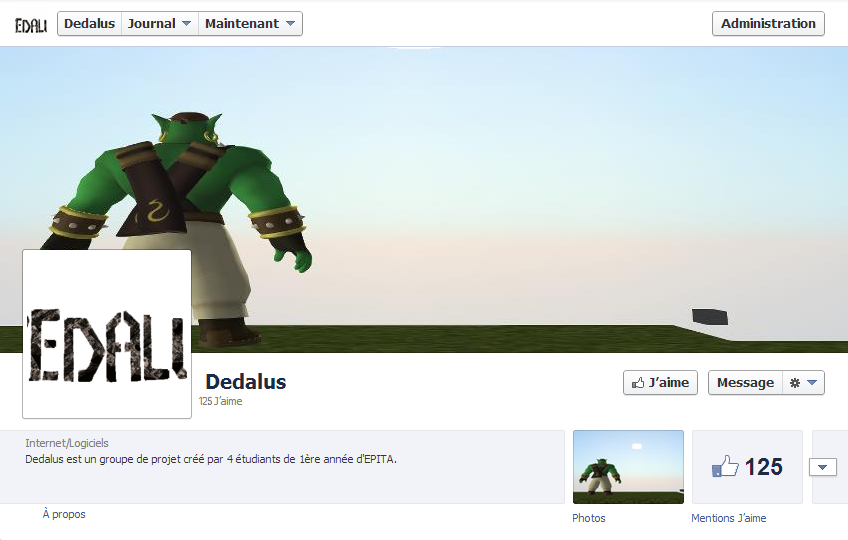
\includegraphics[width = 17cm]{images/fb.png}
				\newpage

			\section{Web site}
				You might have seen it at the last oral presentation, our website was a little bit empty. Knowing that we made some efforts, and completly redesigned the website.\\
				Thus it has now only one page but is a lot more cooler. We are even using AJAX to fetch data from the database and it works fine!\\
				
				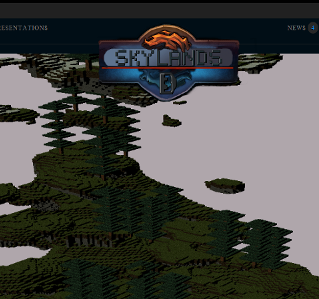
\includegraphics[width = 17cm]{images/website.png}
				
\bigskip
				Querying the database isn't really the same as old plain SQL with Symfony, because Symfony uses Doctrine which uses a traditional SQL base and adds a database
abstraction layer to the database.\\
 Thus with Doctrine, tables are class. Doctrine is mostly a set of PHP libraries primarily focused on providing persistence services and related functionality. Its prize projects are an Object Relational Mapper (ORM) and the Database Abstraction Layer it is built on top of.\\

\newpage
Here is how the database is represented with doctrine :
\begin{lstlisting}
<?php
/* @ORM\Table()
 * @ORM\Entity(repositoryClass="SkyLands\KernelBundle\Entity\NewsRepository") */
class News {
    /**
     * @var integer
     * @ORM\Column(name="id", type="integer")
     * @ORM\Id
     * @ORM\GeneratedValue(strategy="AUTO")
     */
    private $id;

    /**
     * @var string
     * @ORM\Column(name="author", type="string", length=255)
     */
    private $author;
    /**
     * @var string
     * @ORM\Column(name="message", type="text")
     */
    private $message;


    /*Get id
     * @return integer 
     */
    public function getId() { return $this->id; }}
?>
\end{lstlisting}
\newpage
 		Thanks to symfony, creating the file and launching a php command line Symfony will detect all new doctrine class (marked with a @ORM comment) and update the database for us (creating a table).\\
 		Also creating a new row in a table and reading from a table is made easier with doctrine : 
\begin{lstlisting}
<?php
//writting
$article = new News();
$article->setTitle('4th Oral presentation');
$article->setAuteur('Dedalus');

$em = $this->getDoctrine()->getManager();
$em->persist($article);
$em->flush();

//reading
$repository = $this->getDoctrine()->getManager()->
getRepository('SkyLandsKernelBundle:News');

$newsList   = $repository->findBy(array(), array('date' => 'desc'), 4, 0);
//newsList is an array of array access it with newsList[i][fieldName]
?>
\end{lstlisting}

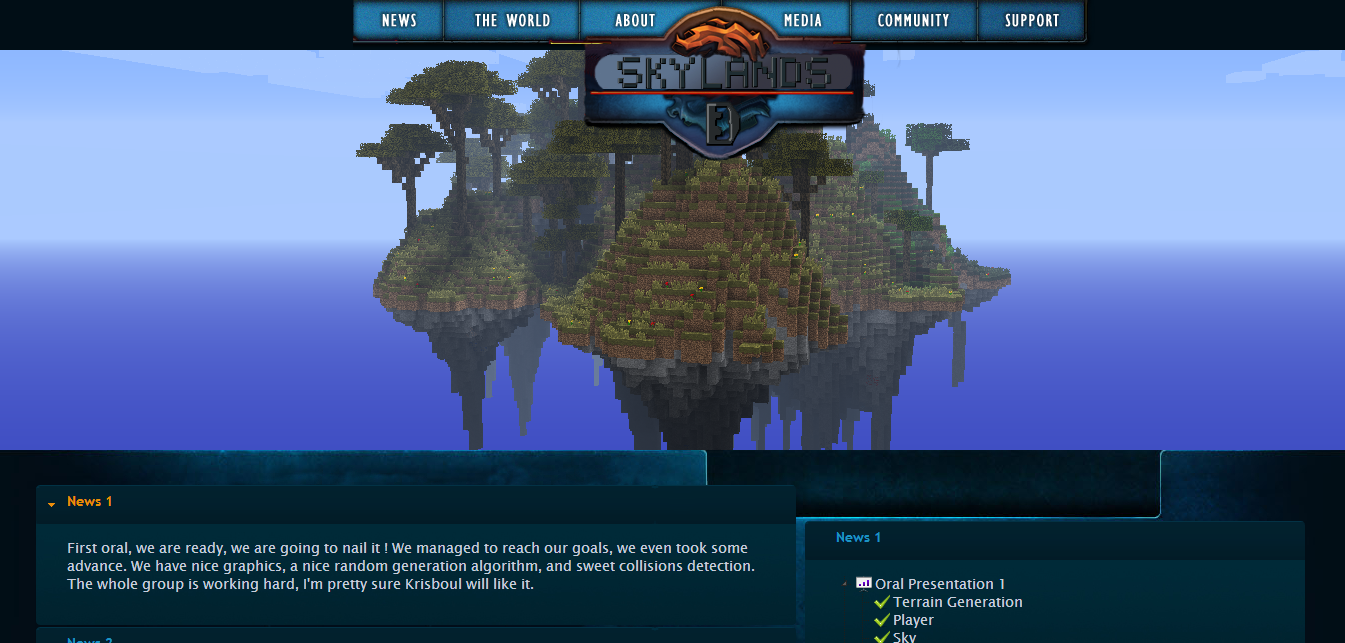
\includegraphics[width=16cm]{images/web.png}

    \chapter{\textcolor{blue}{GUI and Web UI}}
      \section{A windowed Game}
        Following the example given by Minecraft, we decided to give up on a full screen game and go for a windowed game.\\
        This means that users can resize the window in which the game is to any size they want.\\
      \section{A GUI flawed}
        We recently discovered that Mogre, the 3d engine we were using was no longer maintained (and hasen't been for two years) and that it had tremendous flaws!\\
        You already know that Mogre is a .NET wrapper for Ogre (a C++ 3d engine), which means that Mogre is just a ``translator'' however translating from C\# to C++ isn't that easy.\\
        Thus many functions which are in Ogre are not translated in Mogre and therefore, for some special cases, we need to access directly to the C++ functions or use pointers.\\

        For the GUI it was worse, we could get Mogre to display images but never text, and we couldn't do anything about it because of a C\# to C++ error...\\
        We tried tinkering in the source of Mogre but we never could make our way out (they were using a weird procedure, wrapping from C++ to JAVA and the translating the wrapper in C\#).\\
        We tried using some of the new Ogre features which were added in the 1.8 version of Ogre (they are now writing the 2.0 version) however after to translating a few thousands lines of C++ to C\#, without surprise we discovered that the latest version of Mogre (1.7.4) could not work with the new GUI features.\\

        At that moment our spirit was really low, we didn't know what to do and couldn't really continue our Menus without doing horrible things.\\
        % TODO : Si quelqu'un a une idée pour exprimer ce que je veux dire
        However by sheer luck we discovered an awesome library, which allowed us to create Web UI which is just a fancy term for any interface built with HTML, JS, and CSS.
        Awesomium is a library which provides the special sauce that allowed us to integrate Web UI content in any .NET application! \\
        And guess what! The C\# version of Awesomium is just a wrapper of the C++ version!

      \section{A Web UI}
        Finding a way to display our menus and what's more in HTML, CSS and JavaScript was a releif. However we had to completely destroy the old interface and thus rebuild our GIU from scratch. We first had to rebuild the previous GUI (we chose a different theme that time) and then the ingame HUD.

           \subsection{ Main Menu}

    In order for the game to be totally finished, we thought of giving it a very specific and personal style that wouldn't remind the players of any other games. \\

    They also had to match the spirit of the game which is supposed to take place somewhere in space. As a result, all the menus have been recreated: they all now have new skins as well as new features.  \\ 
 
    The Main menu is the only one that didn't changed much: it still links to the ``Play Menu'' the ``Option Menu'' and enables the player to exit the game, but the skin was changed into a spaceship-looking interior. \\

    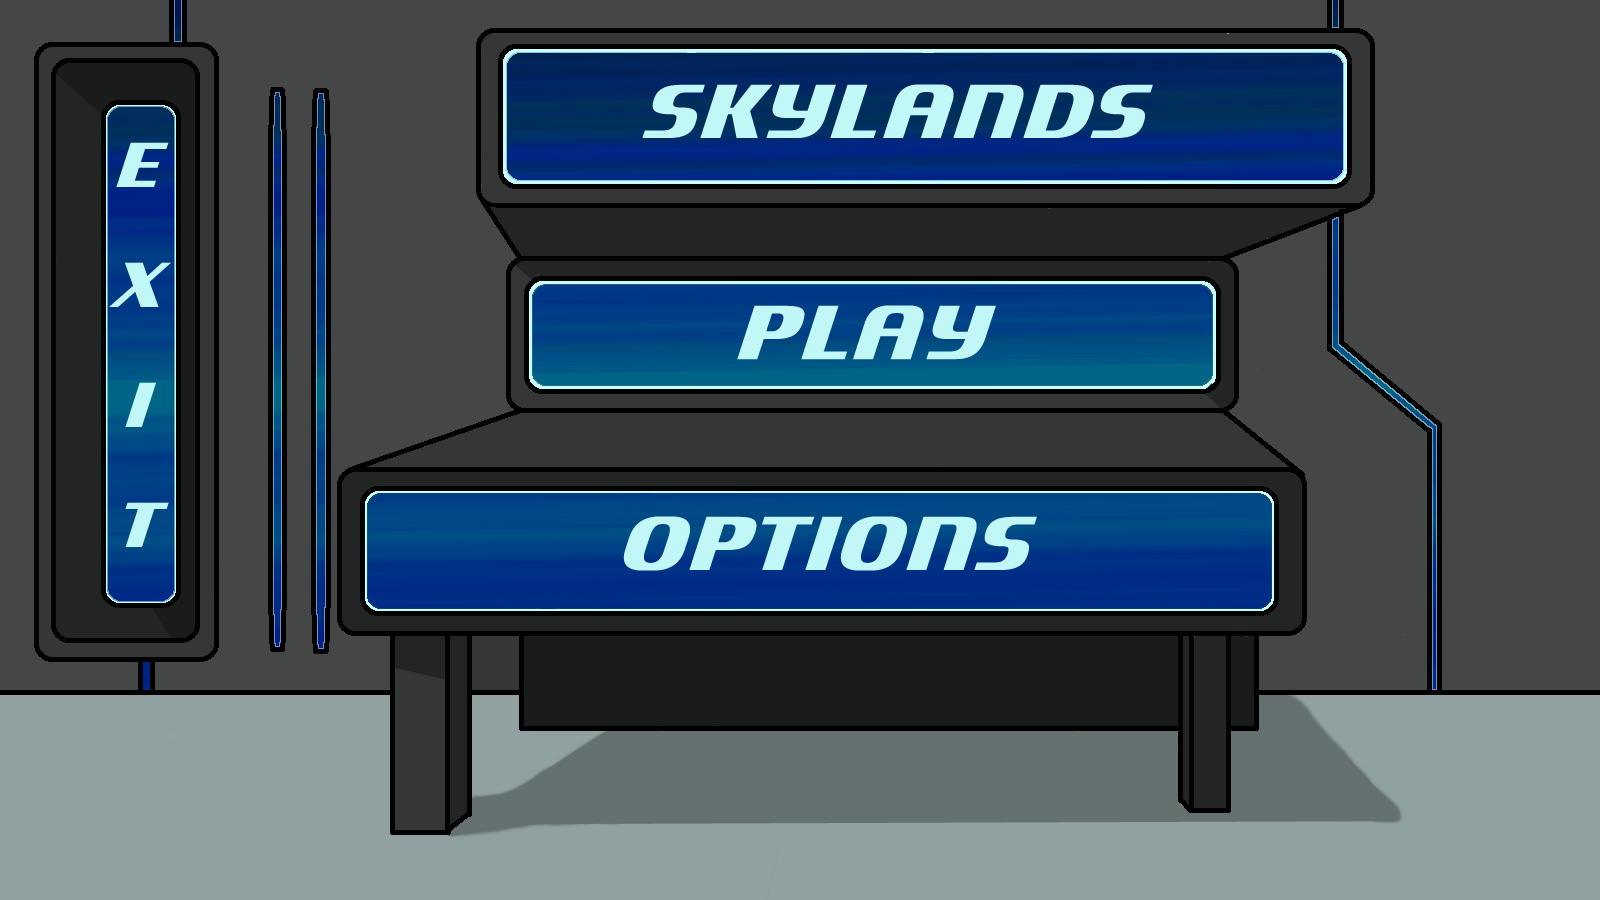
\includegraphics[width=15cm, height=8cm]{images/Menus/Menu_Normal_view.png} 
    \newpage
		\subsection{Option Menu}
    The ``Option Menu'' was also redesigned in the same theme and now let the player chose to enables sound and VSYNC or not and links back to the Main Menu. \\

    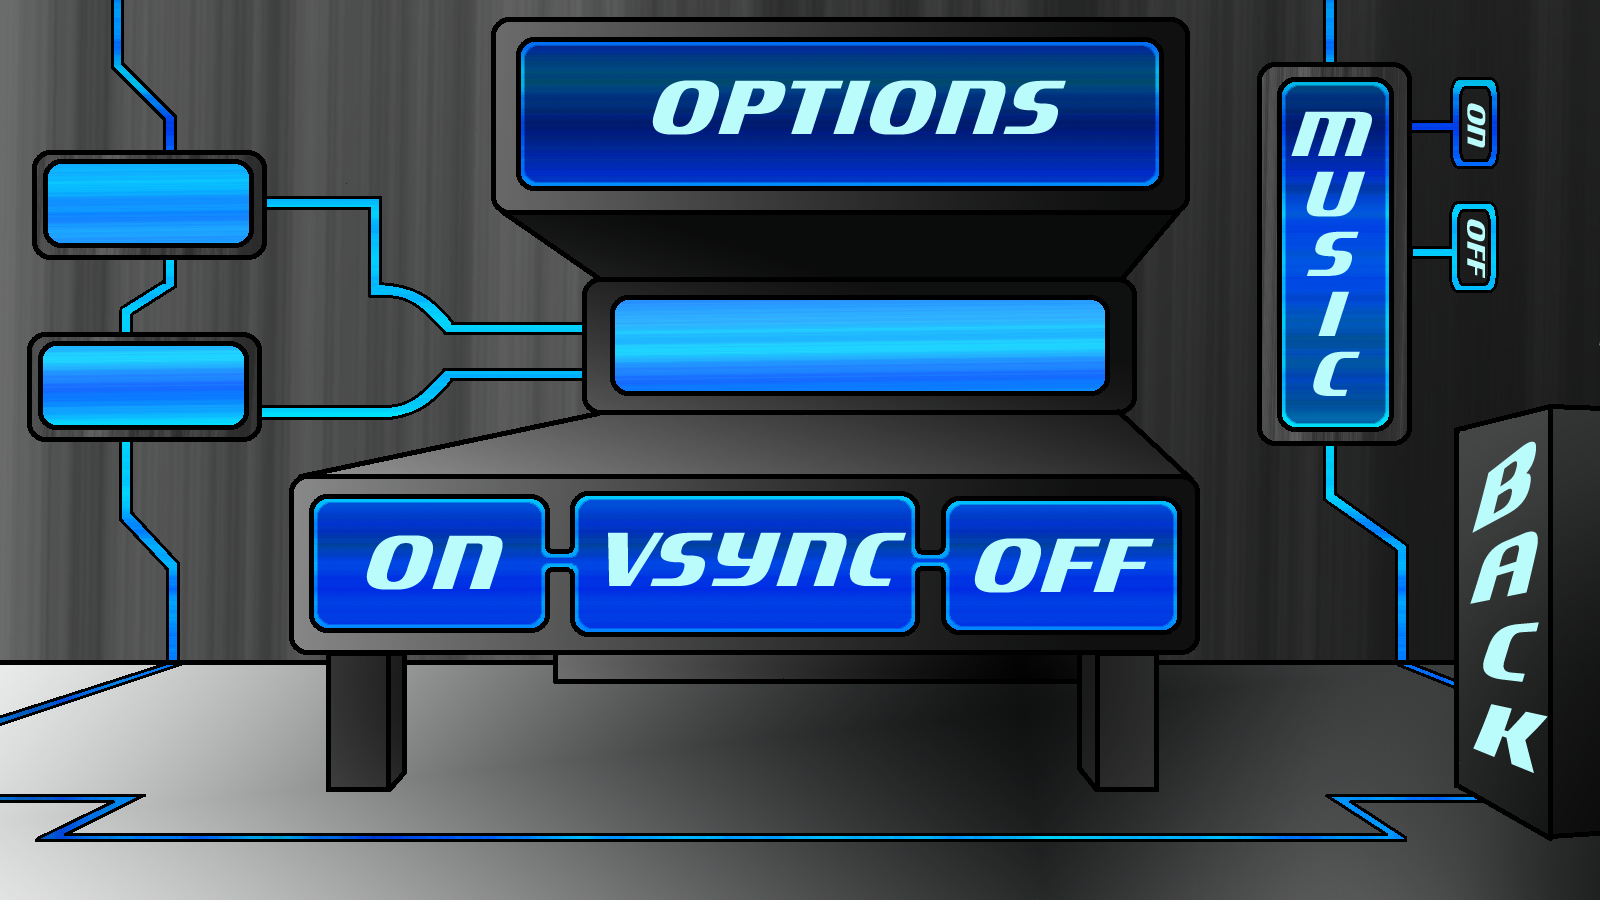
\includegraphics[width=15cm, height=8cm]{images/Menus/Menu_Options_normal.png}

		\subsection{Play Menu}
    The ``Play Menu'' allows the player to load a previously saved game and to access the Scenario Editor. After choosing an existing scenario in the Editor the player can launch the game by clicking on ``Create World''. \\

    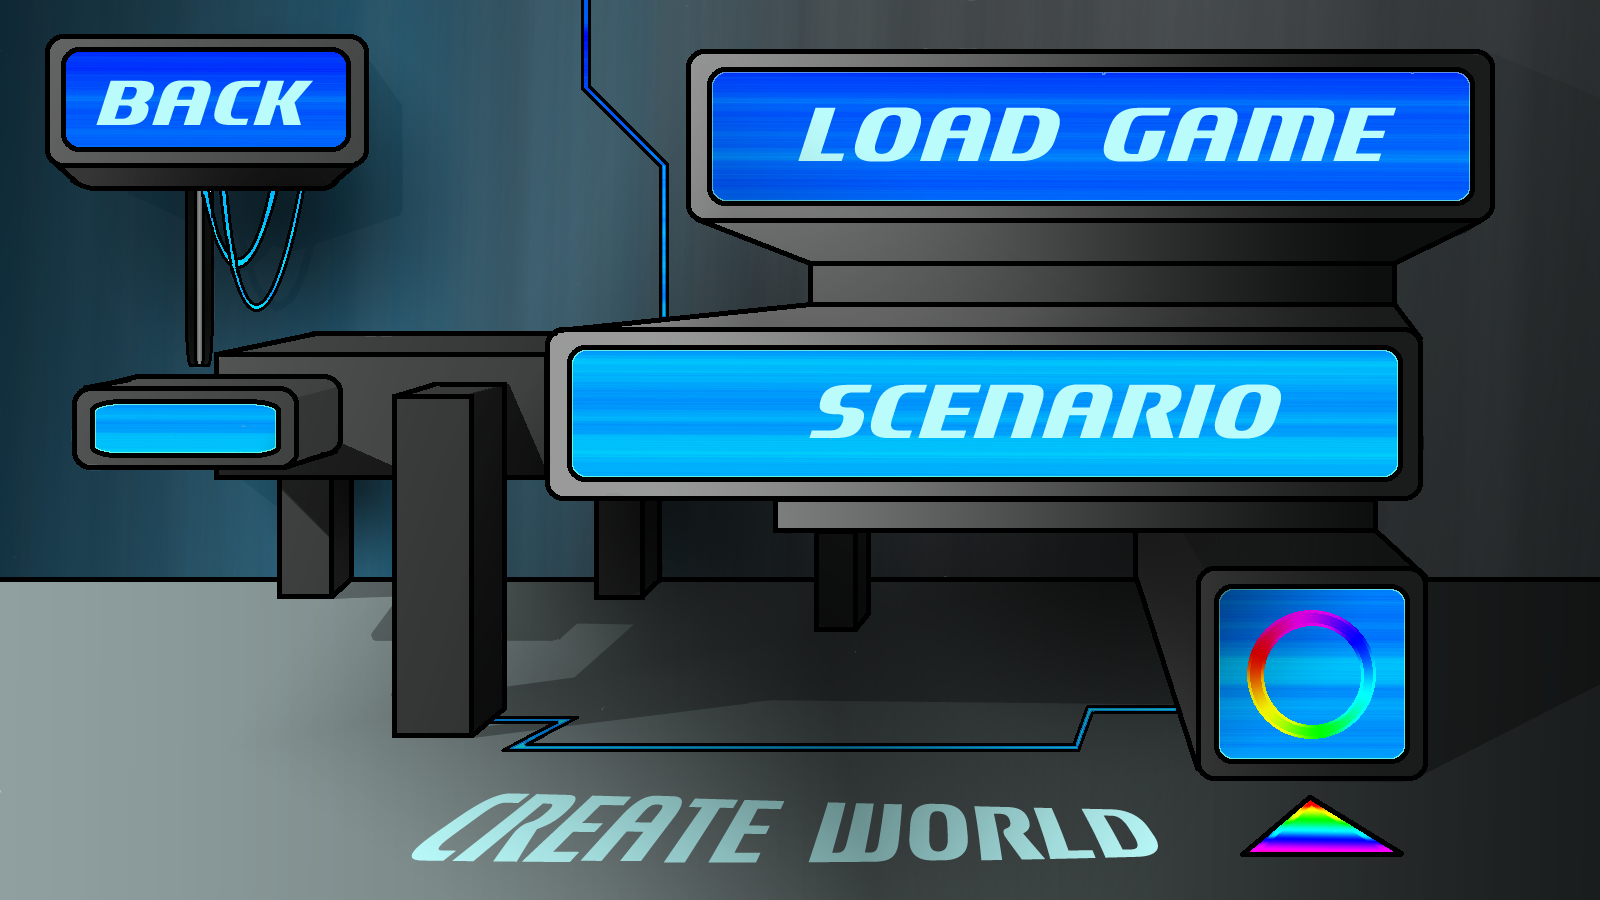
\includegraphics[width=15cm, height=8cm]{images/Menus/menu_play_normal.png}

    \newpage
		\subsection{Scenario Menu}
    The ``Scenario Menu'' is divided in four interactive parts. The middle blue screen let the player choose an existing scenario among those on the scrolling list, then the ``OK'' button will redirect him to the play menu to launch the scenario. The ``NEW'' button as well as the ``EDIT'' button both link to the scenario editor, NEW will let the player create a world from the scratch thanks to the preexisting structures and maps while EDIT will let the player edit a existing scenario.\\


    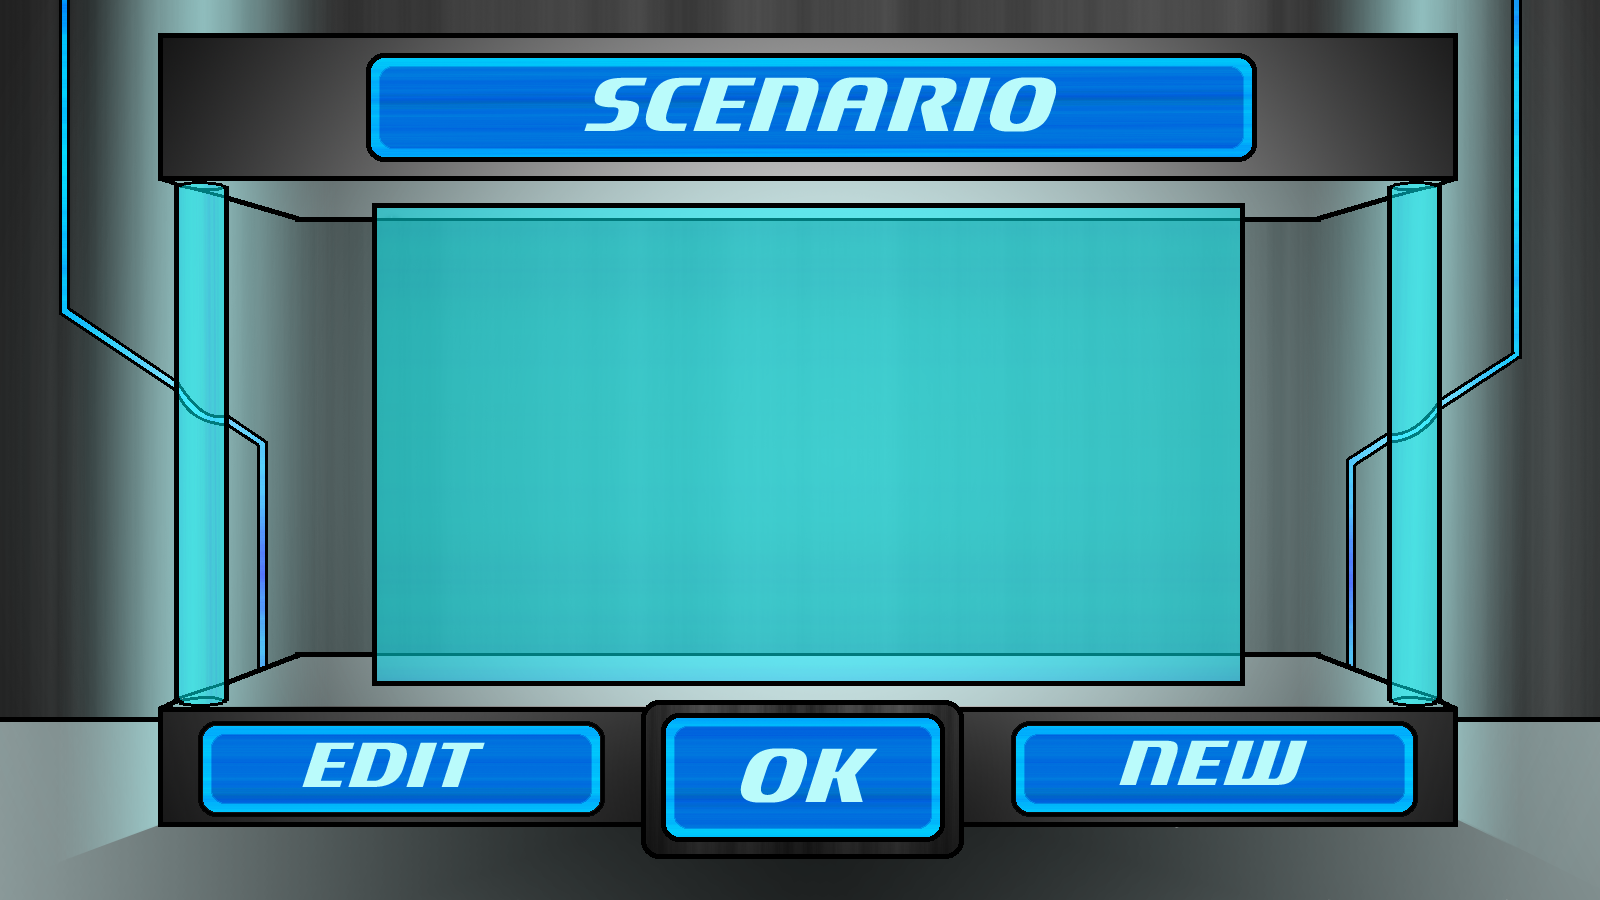
\includegraphics[width=15cm, height=8cm]{images/Menus/Load_scenario_normal.png}


    \begin{textblock}{0.35}(0.47,0.55)
    The Scenario editor is divided in two parts. Left is the editor and right is the created map displayed. \\

The user can choose a preexisting map in the editor by scrolling up and down with the arrows and clicking ``OK'' to edit it.\\

 The editor will then disappear to let the player travel the map in a first person view so that blocks can be added or removed or made into event-blocks. If no map are satisfying, a new map can be created by typing its name in the textbox. \\

``ADD'' will enable the player to add already existing structures on the map like the pyramid or towers.\\
    \end{textblock}
    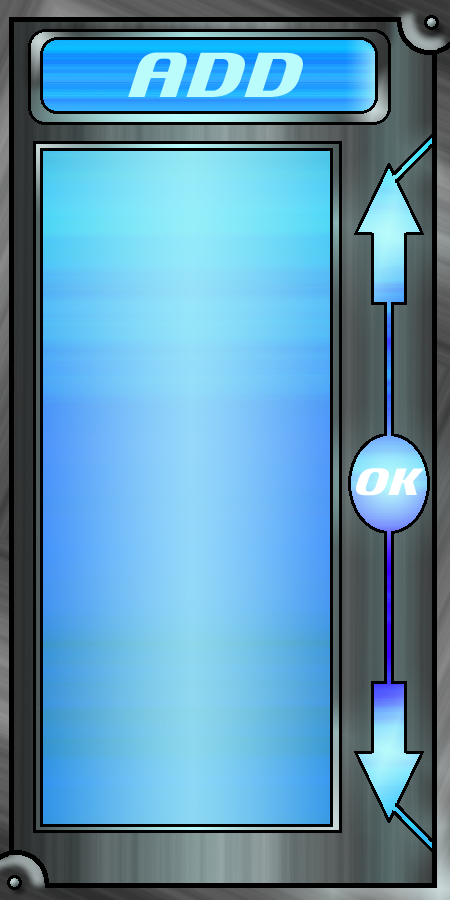
\includegraphics[width=6cm, height=12cm]{images/Menus/Scenario_editor_normal.png}

    \newpage
		\subsection{Ingame Menu}
    Finally, the ``Ingame Menu'' has been recreated too. Apart from its new spaceship-like skin, it now enable the player to save the game, go back to it or go back to the Main Menu.\\

    \begin{textblock}{0.6}(0.3,0.15)
    
    
\includegraphics[width=10cm, height=9cm]{images/Menus/ingame_menu_normal.png}
    
    \end{textblock}

      ~\\~\\~\\~\\~\\~\\~\\~\\~\\~\\~\\~\\~\\~\\~\\~\\~\\~\\~\\~\\~\\~\\~\\~\\

    A ``GAME OVER'' screen was also added, letting the player respawn somewhere on the map or exit to the Main Menu.\\

    
\includegraphics[width=15cm, height=8cm]{images/Menus/death_screen_normal.png}


    \chapter{\textcolor{blue}{Random Terrain Generation}}
      \section{At First Static Terrain}
        At the beginning of the year, the pattern we used for creating islands was very simple and extremely fast.\\
        We applied basic functions as well as more advanced functions such as :

        \begin{itemize}
          
          \item $\sin$ 2d
          \item $\sin$ 3d
          \item $\cos$ 3d
          \item sin(x) cos(y)
          \item sinc 3d (sin(x) / x)
        \end{itemize}

            \begin{figure}[h]
              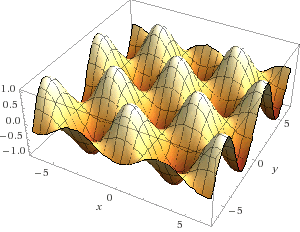
\includegraphics[width=9cm, height=7cm]{images/Terrain/1.png}
              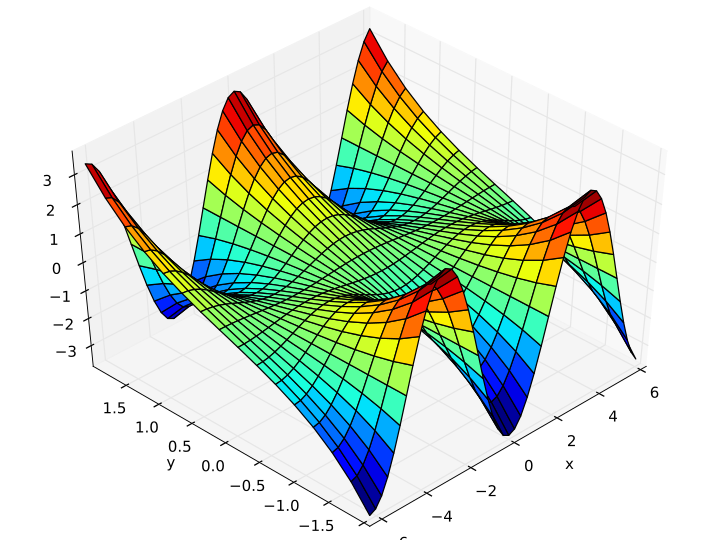
\includegraphics[width=9cm, height=7cm]{images/Terrain/2.png}
              \begin{center}\it The sin(x) * cos(y) and the sinus 3d function\end{center}
            \end{figure}


            \begin{figure}[h]
              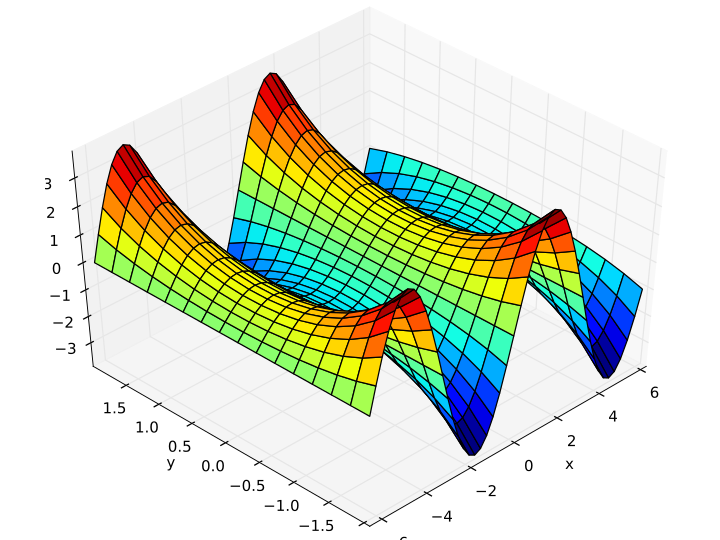
\includegraphics[width=9cm, height=7cm]{images/Terrain/3.png}
              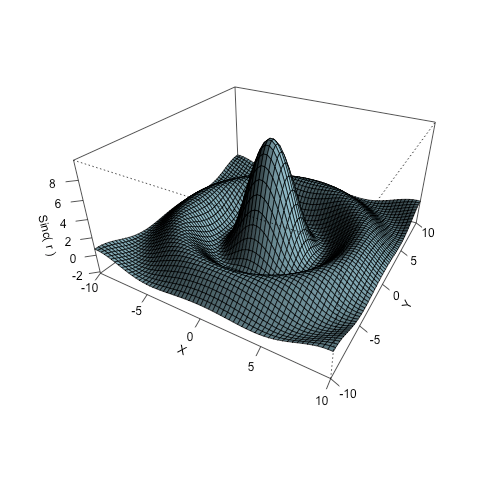
\includegraphics[width=9cm, height=7cm]{images/Terrain/4.png}
              \begin{center}\it The sin(x) function represented in 2d and the sinc 3d function\end{center}
            \end{figure}

            However we quickly understood that using basic functions was not enough. We also wanted random terrain generation however, those functions didn't provide any random factor.\\
            Therefore after some research we ended up using a Perlinh Noise algorithm.
 
      \section{Then Perlin Noise}
        If you look at many things in nature, you will notice that they are fractal. They have various levels of detail. A common example is the outline of a mountain range. It contains large variations in height (the mountains), medium variations (hills), small variations (boulders), tiny variations (stones) . . . you could go on.\\
        Look at almost anything: the distribution of patchy grass on a field, waves in the sea, the movements of an ant, the movement of branches of a tree, patterns in marble, winds. All these phenomena exhibit the same pattern of large and small variations. The Perlin Noise function recreates this by simply adding up noisy functions at a range of different scales.\\

        \subsection{Noise}
          Perlin noise generates coherent noise over a space. Coherent noise means that for any two points in the space, the value of the noise function changes smoothly as you move from one point to the other -- that is, there are no discontinuities.\\

          \begin{figure}[h]
              
\includegraphics[width=9cm, height=7cm]{images/Noise/noncoherent.png}
              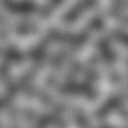
\includegraphics[width=9cm, height=7cm]{images/Noise/coherent.png}
            \end{figure}

          \subsection{Generating Perlin Noise}
            The outline of our algorithm to create noise is very simple. Given an input point P, look at each of the surrounding grid points. In three dimensions there will be eight.\\
            For each surrounding grid point Q, we choose a pseudo-random gradient vector G. It is very important that for any particular grid point you always choose the same gradient vector. 

            Compute the inner product G . (P-Q). This will give the value at P of the linear function with gradient G which is zero at the grid point Q.\\

            When we have 8 of these values. We interpolate between them down to the point, using an S-shaped cross-fade curve (eg: 3t2-2t3) to weight the interpolant in each dimension (we could use a sin function but it would be too slow). This step requires computing 8 S curves, followed by 8-1 linear interpolations (the value has a dimension of degree 1).\\

            We then create an array of the width, height and length of the terrain and fill it with the perlin noise value. We then iterate through the array's 3 dimensions and calculate a noise value for each cells of the array.\\
            The noise value is based on experimentations and advice given by experienced people. In the beginning, the value was computed using a simple linear function, however it is now computed using a polynomial function ad two noise arrays :

            \begin{lstlisting}
              
  double noiseValue = (noise[xx, yy, zz]) * noise2[xx, 255 - yy, zz] + noise[xx, yy, zz] - System.Math.Abs(1 / smoothHeight * (yy - smoothHeight - minElevation + 20))

            \end{lstlisting}

            Where smoothHeight correspond to (maxElevation - minElevation) / 2. The noise value computed is a value between -1 and 1 and if it is lower than 0 we consider that it is air.
      \section{Different Islands}
        The smoothHeight value allows us to make different type of Islands, such as plains or even mountains. Because when smoothHeight's value is High, the values computed by noiseValue are higher and tend to be more scattered whereas low values tend to be more concentrated on one level.

        %TODO : image needed
      \section{Decorating the Islands}
        By default, the terrain is just a big cube of stone. However, when generating it, we add air blocks and, solid blocks under air blocks are usually grass (it can be set to another block).\\
        Since we do not want to iterate through the terrain multiple times, this is done when generating the terrain thanks to little algorithm trick :\\

          \begin{lstlisting}  
            for (int xx = 0; xx < this.mIslandSize.x; xx++) {
                for (int zz = 0; zz < this.mIslandSize.z; zz++) {
                  for (int yy = Cst.MAXHEIGHT; yy > 0; yy--) {
          \end{lstlisting}

            We create the terrain from the top, which allow us to check for each block if it's under an air block and if that's true, place a block of grass.\\
            In case the block we just created is solid, we calculate it's distance from the surface and if we told the program beforeHand that there was a special block at the block's particular depth then the type of block will be the one we set, else it's stone.\\
            %TODO : image needed
            Thus in most of the Islands, the first layer is grass and the next two are dirt. The height and the layers are set in a class called Biome.\\

          Once we finished generating the terrain, the next step is to populate it. Which means to add trees or cactus in the different biomes.\\
          Basically we choose a random x and a random z and look for the highest solid block. We then add the cactus and trees.  
      \section{Structures}
          The different structures are usually specific to the biomes and are generated procedurally. As for the cactus and the trees, we get a random point and add the structure.
          We have multiple structures :
          \subsection{Pyramid}
            The pyramid is a simple structure that contain a portal that gives us the possibility to travel from an island to another. Pyramids can obviously be found only in the desert.
	\begin{center}
           	\includegraphics[width=8.5cm]{images/Pyramid.png}
          \end{center}
          \subsection{Caverns}
            We have also implemented caverns. These are holes that you can find in the mountain biome, and they uselly contain a portal. The caverns give the game a bigger solo gameplay, since they are only accessible by the player, and not by his robots.
          \subsection{DarkTower}
        \subsubsection{Introduction to the dark tower}
          The dark tower is the biggest structure we made, it is composed of four main towers floating in the sky and is part of the plain biome. This structure is huge because it size can reach 362 blocks on the y axis and has almost 41 floors

        \subsubsection{The main buildings}
          The tower consists in four main buildings whose height vary between 60 and 88 blocks it has about seven floors which can be climbed using the arcane levitator which as it names implies allows you to levitate. Basically if you are on the levitator, it will lift you up to the next floor.

          \begin{center}
            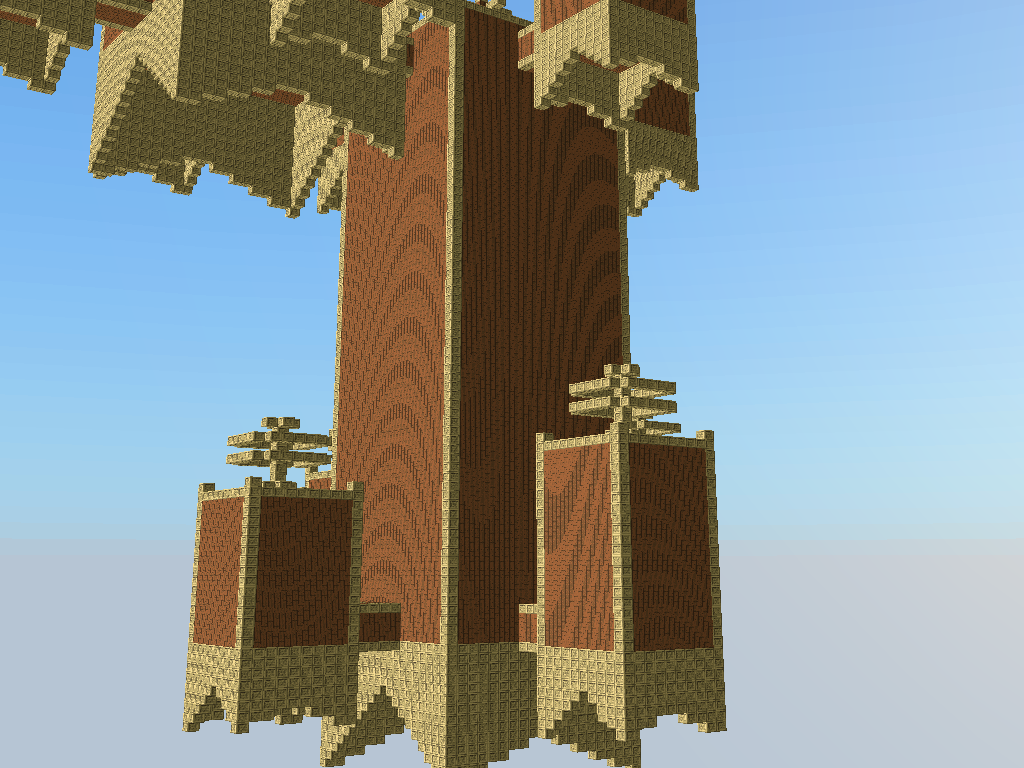
\includegraphics[width=7.5cm]{images/DT/Main.png}
            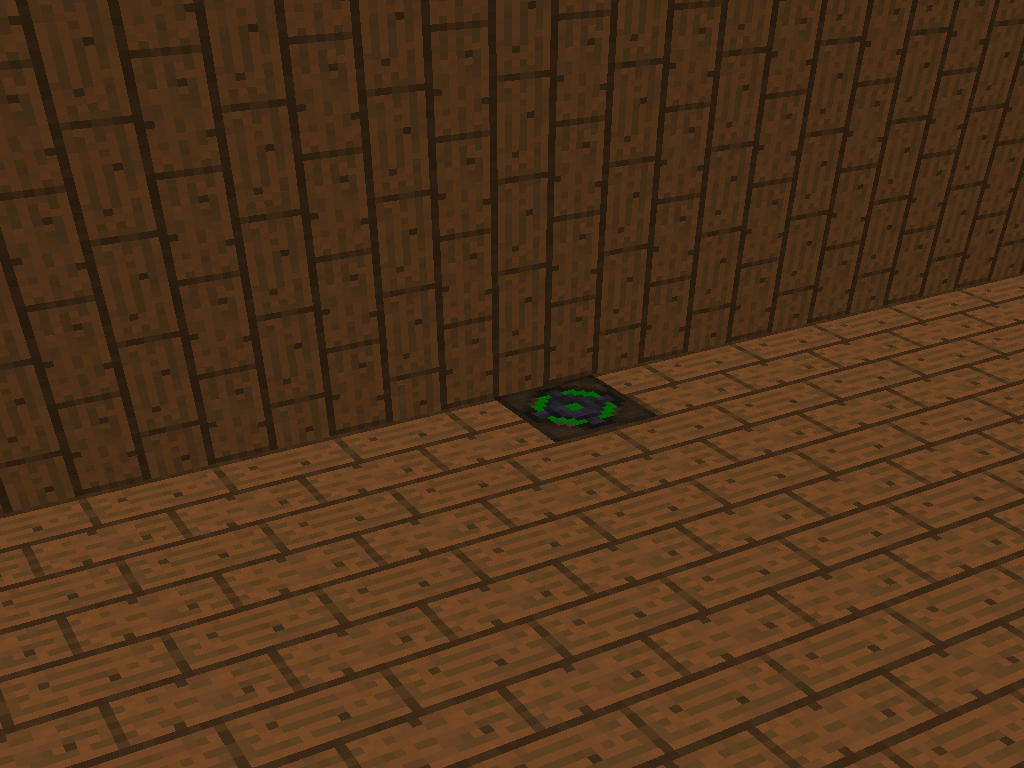
\includegraphics[width=7.5cm]{images/DT/floor.png}
          \end{center}
        finally on the first and last floor of the main tower, bridges connect the main towers to medium towers or another main tower.

        \subsubsection{Bridges}
          Bridges are generated only by the main towers and allows the player to continue climbing the dark tower. One difficulty we encountered while ``building'' the tower was the orientation. Indeed, the algorithm to build a bridge facing north is not the same as the algorithm to build a bridge facing west. We struggled to find a way to ``unify'' those algorithm but we finally choose the simplest solution using a switch. Here is the result :
          \begin{center}
            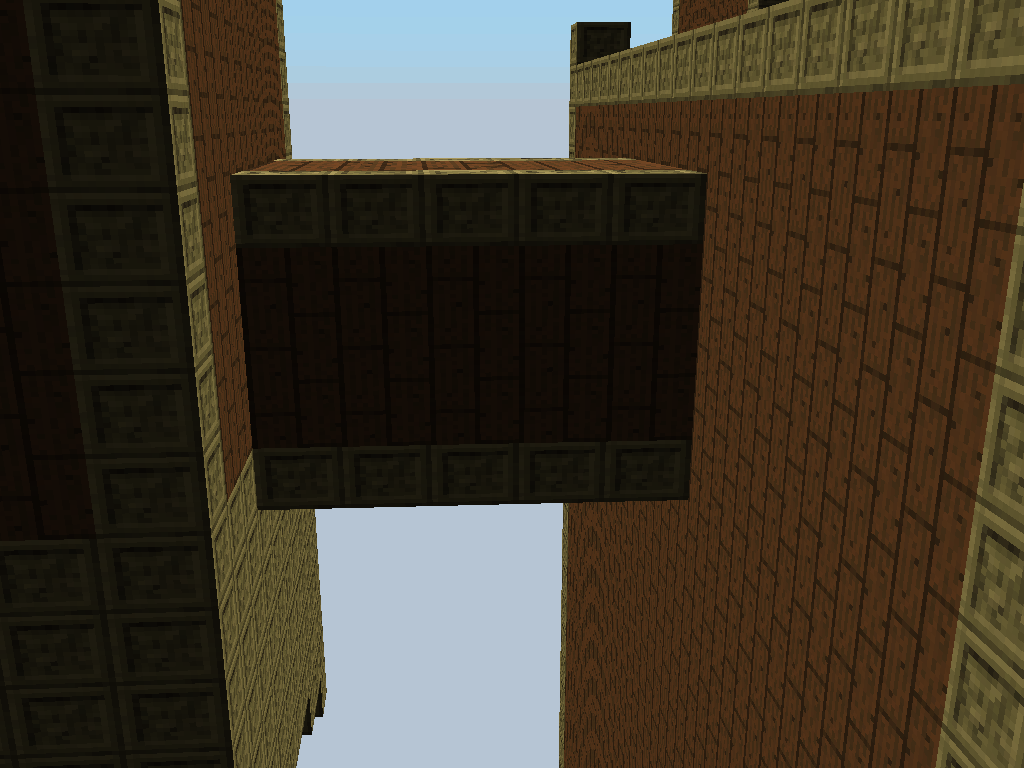
\includegraphics[width=7.5cm]{images/DT/bridge1.png}
            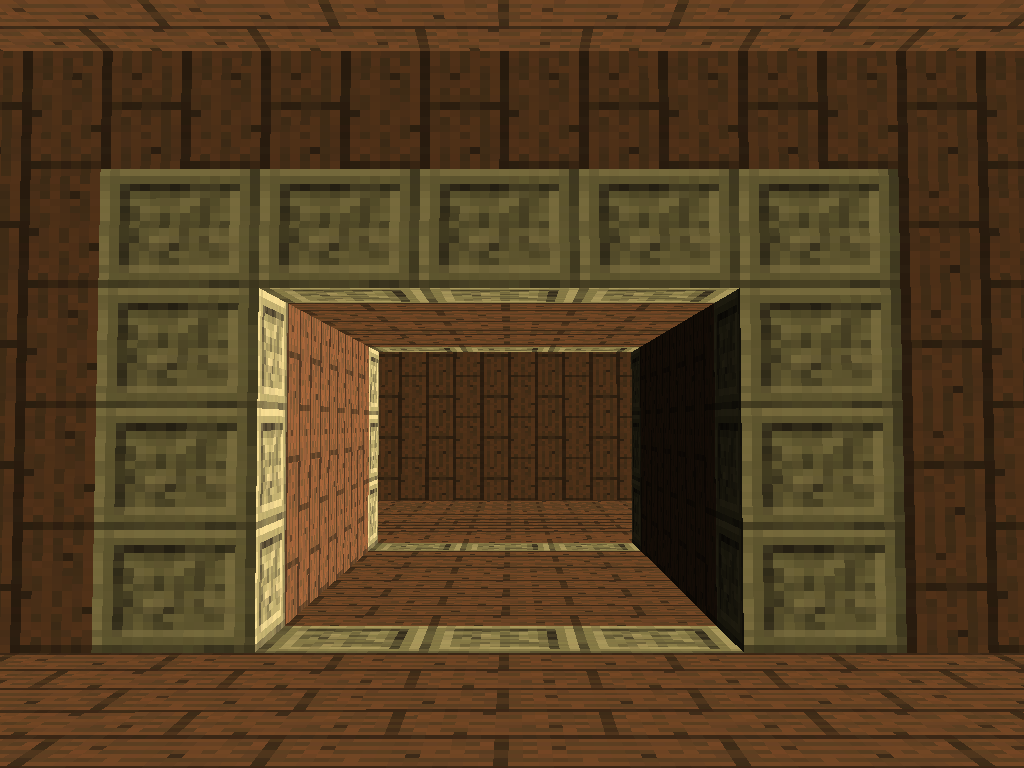
\includegraphics[width=7.5cm]{images/DT/bridge2.png}
          \end{center}

        \subsubsection{Lower towers}
          As I've already said before the main tower are linked by bridges to lower towers their height vary between 15 and 30 blocks and in most of them, the player will find prisoners unit guarded by enemies and when they are defeated (the enemies), the prisoners joins the player which can then command them.
          \begin{center}
            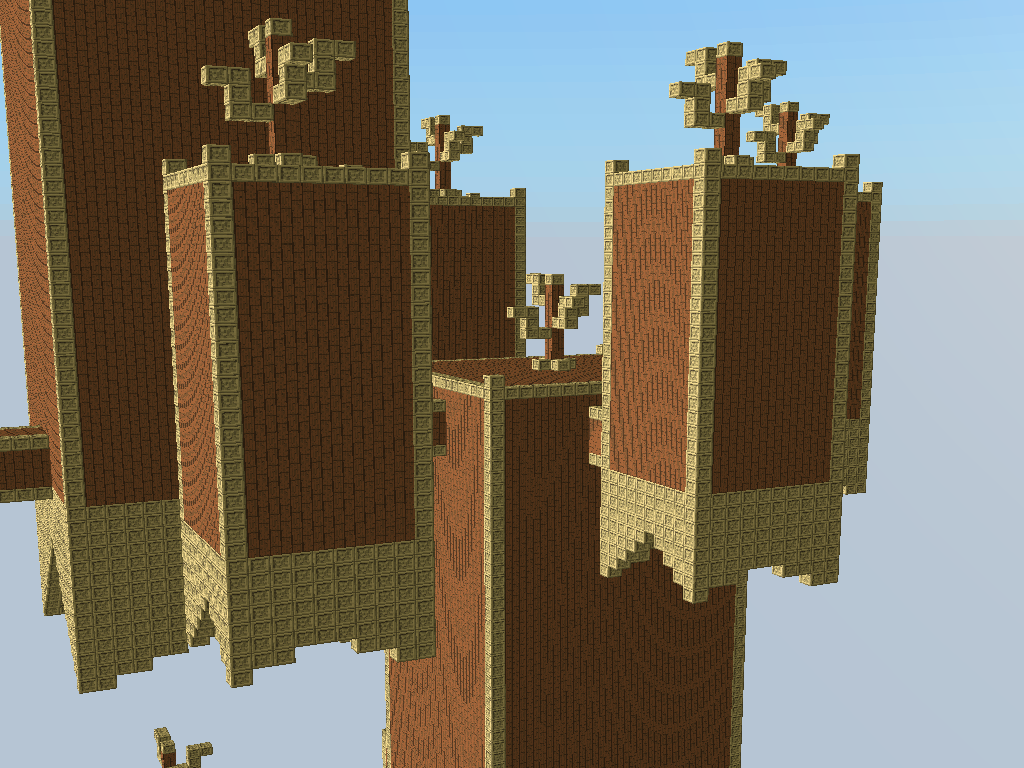
\includegraphics[width=7.5cm]{images/DT/mediumTowers.png}
            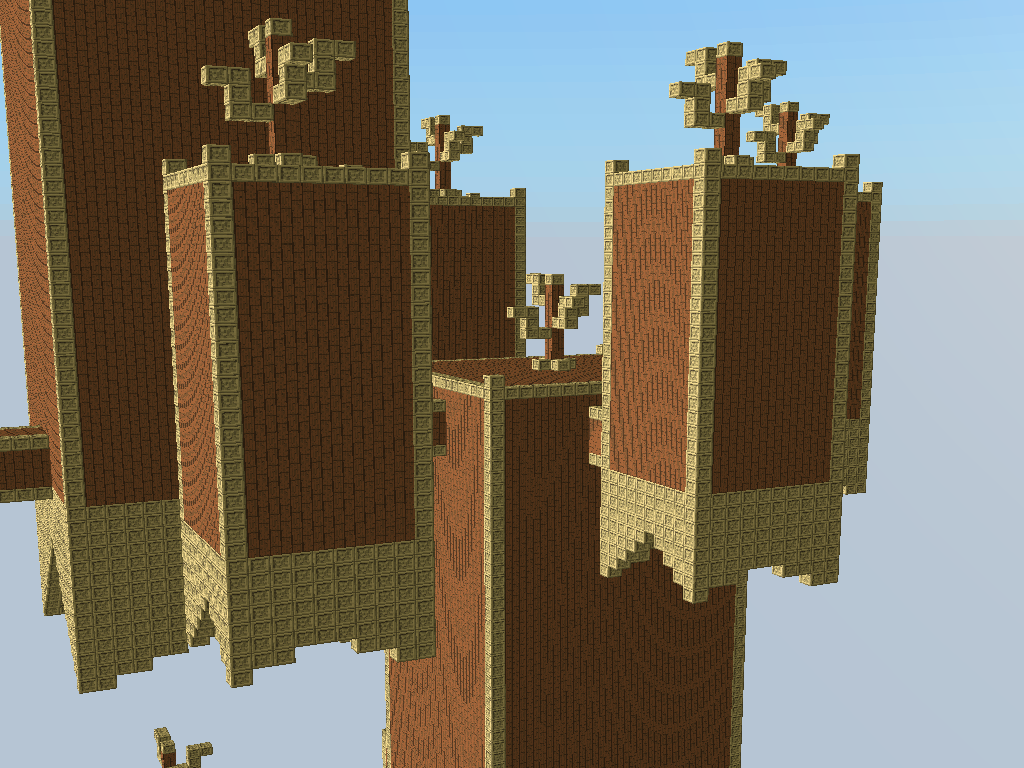
\includegraphics[width=7.5cm]{images/DT/mediumTowers.png} %TODO : Robots
          \end{center}

        \subsubsection{Roofs}
          Among the multiple things which make the tower, one of the most beautiful thing are the structures on the roof, we made 3 of them :
          \begin{center}
            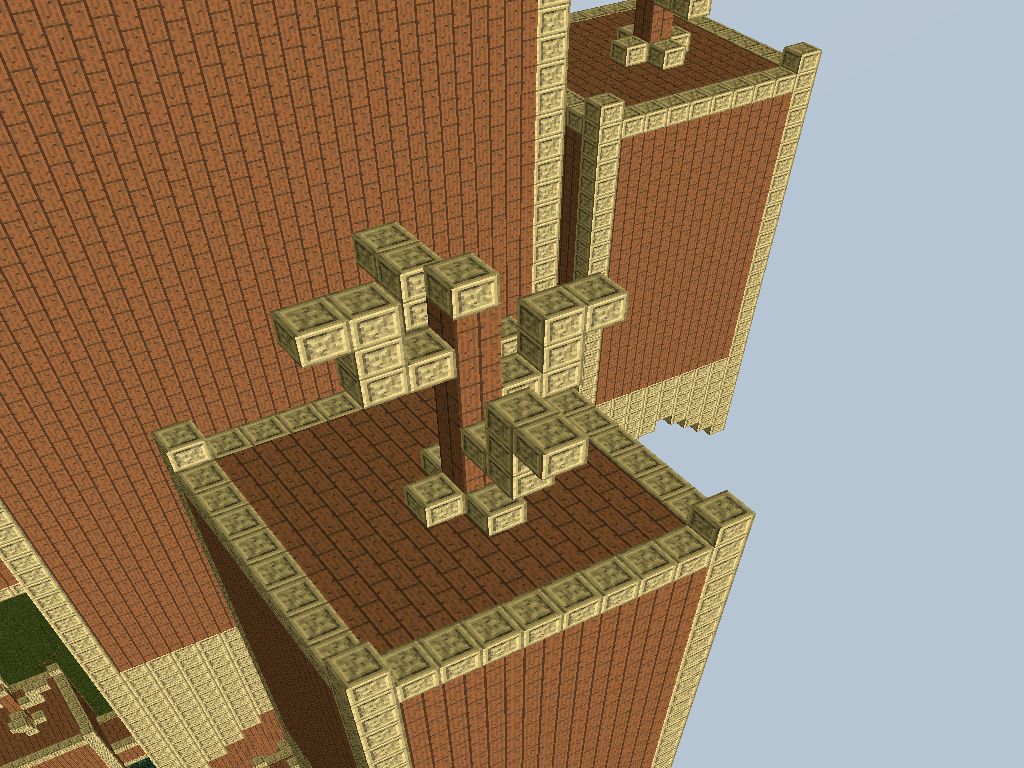
\includegraphics[width=5cm]{images/DT/roof1.png}
            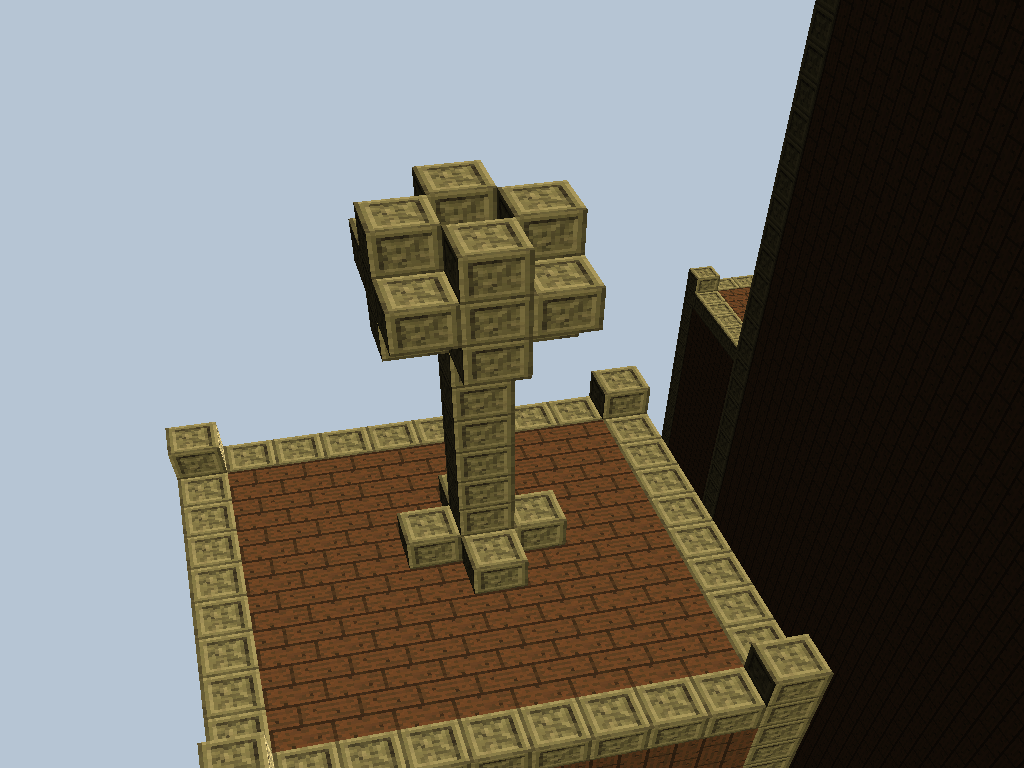
\includegraphics[width=5cm]{images/DT/roof2.png}
            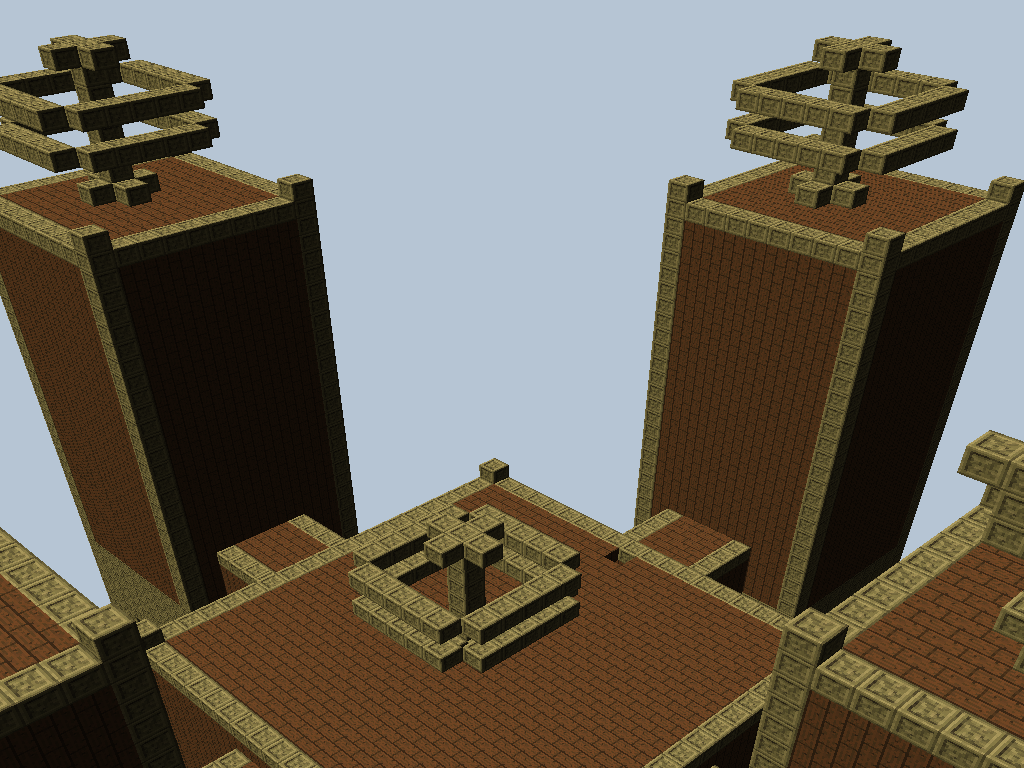
\includegraphics[width=5cm]{images/DT/roof3.png}
          \end{center}
        \subsubsection{DarkBeard}
          Finally, we had to deal with the bottom of the towers. At the beginning we thought that it would stay flat but, we managed to find a function that made the bottom look amazing. We called it the dark beard.

          \begin{center}
            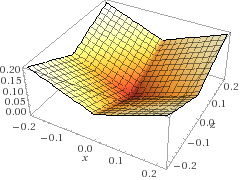
\includegraphics[width=7.5cm]{images/Abs.png}
            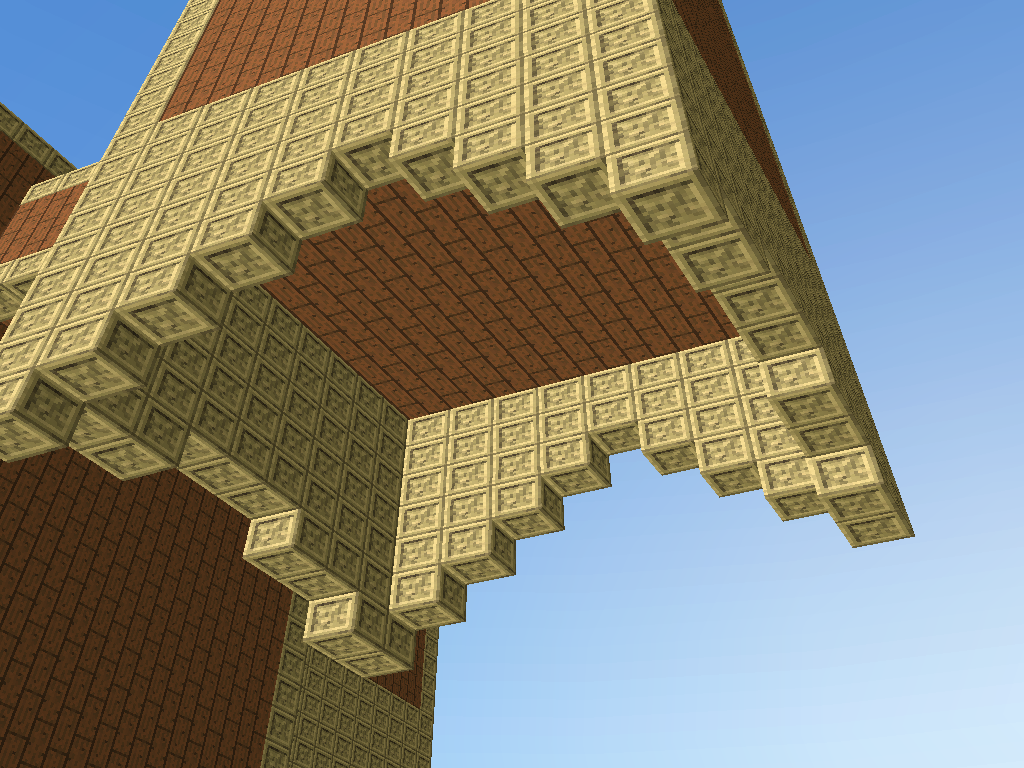
\includegraphics[width=7.5cm]{images/DT/DarkBeard.png} %TODO : Robots
          \end{center}
      \section{Displaying}
        \subsection{Displaying Cubes}
          At first, we thought of displaying cubes which where imported entities from blender. \\
          Of course we only displayed visible cubes (cubes which had other cubes adjacent to all his sides were not visible). However the result was a mere 1 to 10 Frames Per Seconds with a 40 by 40 blocks terrain. In other words a ridiculous amount of Frames Per Seconds.\\

          This lag was mostly caused by the fact that when displaying an entity on the terrain, all it's faces are visible even the ones which you can not see.
        \subsection{Displaying Only Faces}
          Because of the lag caused by this method, we had no other choice but to find another way of displaying the terrain.\\
          Thus we came up with the following idea :\\
          We created in the code the six different faces which are composing a block.\\
          Thanks to Ogre, this was a fairly easy process, creating an object with little triangle composing it in the code is no more than seven line!
          \begin{lstlisting}

ManualObject block = new ManualObject("name");
block.Begin("texture here", RenderOperation.OperationTypes.OT_TRIANGLE_LIST);
    block.Position(new Vector3(0,   0,     0));
    block.Position(new Vector3(0,   100,   0));
    block.Position(new Vector3(100, 0,     0));
    block.Position(new Vector3(100, 100,   0));

    block.Triangle(0, 1, 2);
    block.Triangle(1, 2, 3);
block.End();
        \end{lstlisting}

        Of course there are other things we have to do such as specifying the coordinates of the textures or the normals (normals are used in order to cast shadow on the surface).\\
 
        Once the six different faces were created, we would iterate through the terrain and each time we would find a visible face (face that is not hidden by another block), we would make a copy of the created face, assign it a texture and then, place it at the correct position.

        \begin{center}
            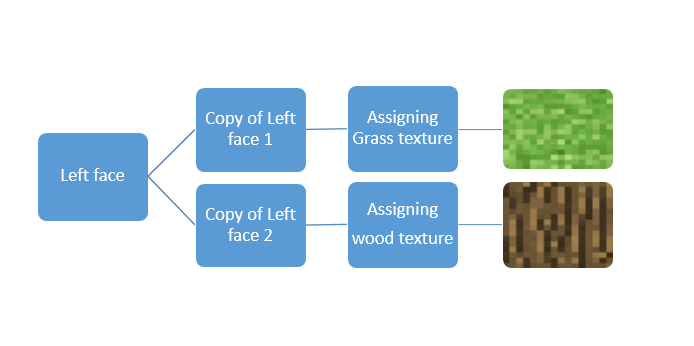
\includegraphics[width=16cm]{images/Display.png}
        \end{center}

        With this system, we ended up having better Frames Per Seconds than the previous displaying system, but this count was very variable and depended on how many entities were displayed on the screen.\\
        
        Basically the the terrain we could display was bigger, but we needed to stop displaying entities at a certain distance (usually 3000 pixels) and our terrain couldn't bigger than 12 chunks of 16 blocks.\\

        Frames Per Seconds were usually between 15 and 30, and as you might expect, we were a bit disappointed because under 24 Frames Per Seconds, animations are uneven or worse ``choppy'' movement or animations, and the frame rate was more often under 25 than above.\\

        \subsection{A better display system}
          Though we had a ``working'' display system we wanted it to be better, we also wanted higher Frames Per Seconds. Actually the moment we made the second we were already thinking of a new algorithm.\\

          The basic gist of it is as follows : we create a ManualObject (as defined higher) in which we don't add any point for each different textures.\\
          We then iterate through terrain looking for visible faces. When we find one, we add, the face to the manual object corresponding to it's texture.\\
          Once we finished iterating through the terrain, we close each manual object (by calling the End() method) and then display them.\\

          Basically, each visible faces with the same texture of the terrain are part of the same material. Thus, instead of thousands of entities (1 per visible face) we only have about 20 entities displayed at all times on the screen.\\

          The end result is, terrain of about 121 chunks for plains Biomes and maximum 2000 (mostly for the mountain biome) with an average frame rate of 60 on Epita's computers!\\

          This system is of course more complicated than explained and has consequences on other parts (especially adding and removing blocks), but it was totally worth the cost, we increased the maximum  frame rate by 30 (sometimes more). Also, the Islands size were tippled, getting from 4*4 to 12*12 (on the x and z coordinates) and can even be increased to 30 * 30.\\
          This means that if we assimilated the terrain as one continuous layer of block (with a height of 1) we would have : 30 * 30 * 16 * 16 = 230400 cubes, counting only top faces and bottom faces : 460800 faces and 921600 triangles, thus around 1 000 000 triangles (with about 60 FPS since the height is only 1).\\
          And we believe we could display even more cubes!\\

      \section{Save and Load}
        Saving and loading the terrain would've been too easy if we had chosen to write it in a text file!\\
        Basically we iterate through the terrain with 3 for (x, y, z) from 0 to the max size and we only need to write the id of the block, which is a byte.\\
        The only thing we need to do is at the begining of the file write the max-size in x, the max-size in the and the max-size in y. Once this is done, we iterate through the terrain using a FileStream and it's method WriteByte.\\

        As for the reading part, obviously we begin by reading the max-size values in x, y, z and once this is done, we iterate through the file using ReadByte and build the terrain according to the input we read. Nothing really technical!\\
      
       The results talk for themselves, for 100 000 blocks = 100 000 bytes = 100 ko. which would be around the number of blocks contained in a 15 * 15 island. So tiny files for big Islands!\\

    \chapter{\textcolor{blue}{Physics}}
      \section{Collisions}
For the second presentation we implemented the physics in our game. At first we included a physic engine called MogreNewt. Even thought it was functional, there was many drawbacks\\

  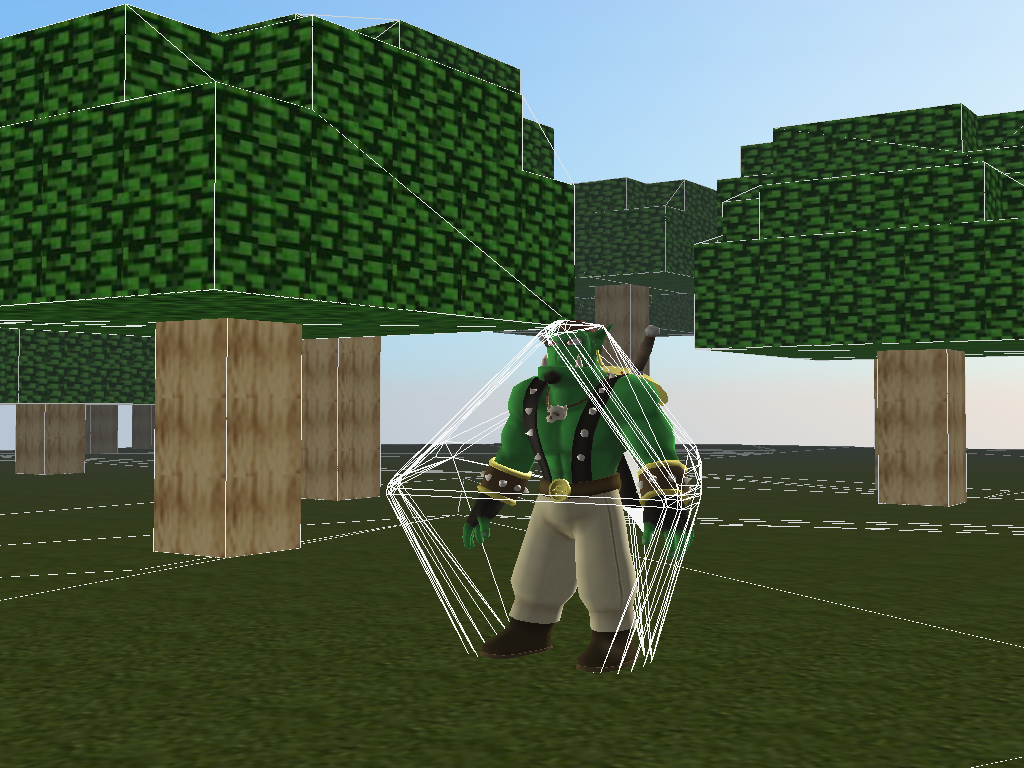
\includegraphics[width=15cm]{images/Physics/MogreNewtWires.png}
\begin{textblock}{0.4}(0.30,0.86)
The wires used for the collisions by MogreNewt
\end{textblock}
\newpage
 Indeed the collisions were too rough, the characters kept on falling in the ground and were then shaking a lot.
This physic engine was clearly not build for a game like our : we hadn't enough control one the collisions events. For instance we simplified the character bounding box by a cylinder.
Then even when this character wasn't moving, it was slowly falling. It wasn't falling on the y axis (in the ground), but it was rotated of 90 degrees instead. So basically he was rolling on the ground (since it was a cylinder).
That's clearly not what we wanted and we couldn't get around this issue in anyway.

Besides, we noticed an important loss of fps which was entailed by MogreNewt. Considering that our game is represented by blocks it would be a shame to use a whole real physic engine. It wasn't planned in our book of specifications to code that but we preferred to do it ourself anyway.\\

\bigskip
  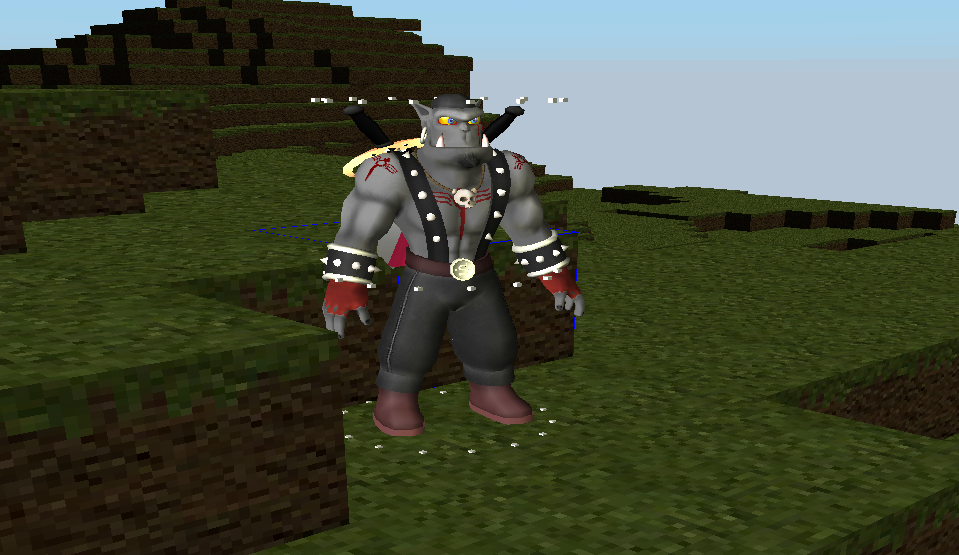
\includegraphics[width=16cm]{images/Physics/HitPoints.png}
\begin{textblock}{0.4}(0.4,0.62)
The hit points we now use.
\end{textblock}

\bigskip\bigskip\bigskip\bigskip

The first goal was to compute the collisions on the y axis only. The main idea was at first to find the position of the feet. We only know the position of the node which is usually (but not always ...) the center of the mesh. From this position we had guess the feet position and after many tries we eventually obtained a satisfying result.
From this position we can compute the result of each translation. Before actually applying the translation, we look at the type of block there are under the feet. But we mustn't look at only one block. Event if the characters are one block width, there are most of the time on 4 blocks at the same time.
To obtain an accurate enough collision, we place a circle of points around the feet position. Depending on the number of points that aren't on any ground, the character is whether falling or not.\\
\bigskip

The y axis collision wasn't a big deal compared to what I called the yaw collision. It's actually as you can guess the collisions on the x and z axis, I call it yaw because it only depends on the yaw angle (that is to say the rotation around the y axis). It was a much more pain since we're in a 3d world and rotations are represented by 4 dimensional vectors : the quaternions Hopefully if we decompose the rotation around the 3 main axis, the problem becomes easier. Once we've managed to compute the yaw angle, the idea is the same than for the y collisions. Each frames, we simulates the movement and check which points are in a block.Then we can recompute the exact collision so that the collided point comes just next to the block.

      \section{Falling, jumping and ... levitating}
		\begin{center}
		  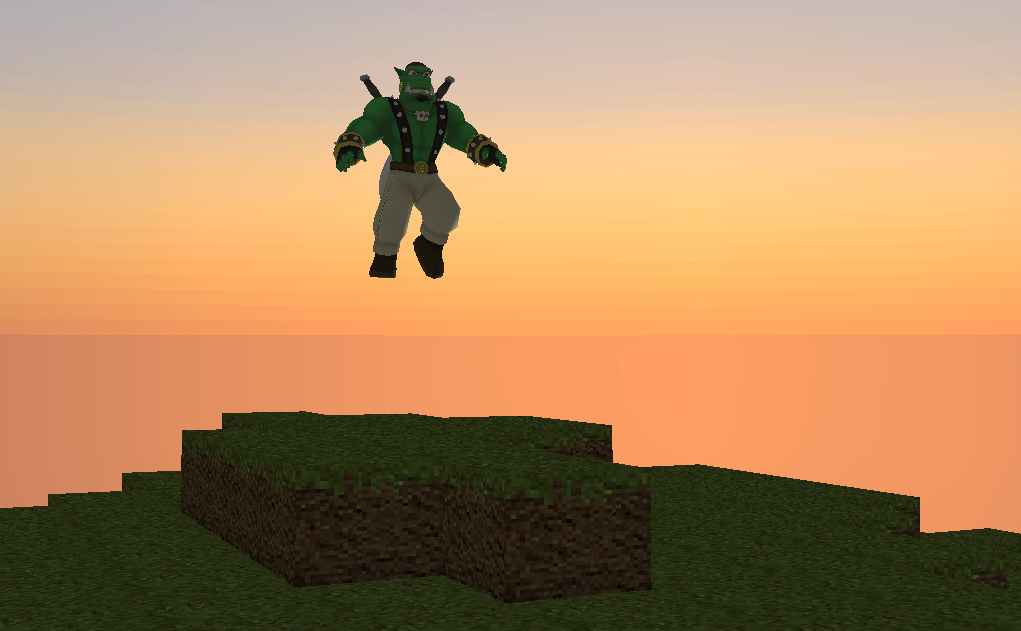
\includegraphics[width=14cm]{images/Physics/SinbadJump.png}
		\end{center}
	The speed on the y axis is compute by a timer. The acceleration follows a squared function depending on constants which are the intial acceleration, the time before the max acceleration and the value of this max acceleration.

Since there is now magic in Skylands, the player can levitate using either the levitating blocks or its own ability. The levitation seemed very important considering the size of the terrain and the abruptly of the mountain for instance. It might come handy during a bad fall ...

      \section{Shoot}

 \begin{textblock}{0.4}(0.120,0.66)
  For the third oral presentation, we implemented the shoot for the player. He can throw cubes at his enemies. There exist 3 different types of cubes fire, water and magic, they inflict more or less damage depending on the enemy.\\

The player can keep the main action button pressed to grow the cube in the hand. Of course the bigger it is, the more damage it will do ! After a few seconds or when the main action button is released, the cube will be fired.
Basically, it follows a right computed from the actual player camera's orientation. It uses rays on his way to determine if there has been a collision and with what kind of entity.\\
    \end{textblock}

    \begin{textblock}{0.6}(0.53,0.66)
    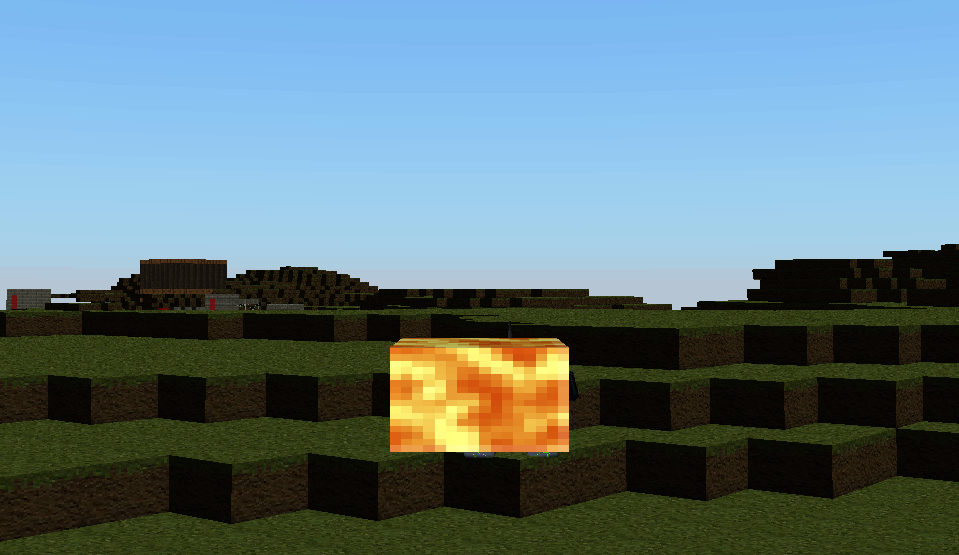
\includegraphics[width=9cm]{images/Physics/FireCube.png}
    \end{textblock}
\newpage

Now the player isn't the only one to be able to fire. There are robots which can be either allied or enemies. In both cased the robots are able to shoot at the closer target there is. The shoot of the robots is quite different. It had to be simpler than a cube that can be hold in position and growth because they are simple AIs.\\

   \begin{textblock}{0.6}(0.120,0.19)
    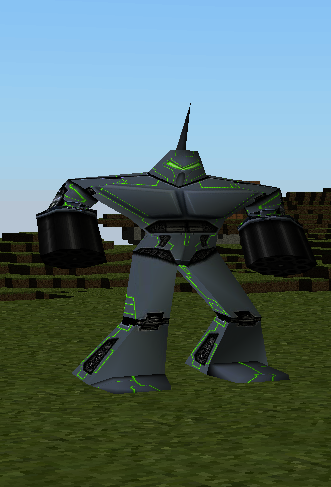
\includegraphics[width=6cm]{images/Physics/RobotShoot.png}
    \end{textblock}

\begin{textblock}{0.4}(0.5,0.19)
Besides we have to think of our fps. We simply couldn't add as many moving cubes as there are characters. Plus the ray is used to compute the collision accurately but it isn't needed if the shooter is a robot. Indeed his shot will be accurate as hell and once he has fired you would better pray that you weren't its target : their shots are unavoidable !\\

But you do can hide before they shoot at you. The blocks between you and the robot will stop the bullet that's why the robot won't event try to shoot. 
Also the bullets are simpler than the player one's. Instead of a cube it's just a line so that the fps are preserved even if many robots will be spawning. 
    \end{textblock}
\bigskip\bigskip\bigskip\bigskip\bigskip\bigskip\bigskip\bigskip\bigskip\bigskip\bigskip\bigskip\bigskip\bigskip\bigskip\bigskip\bigskip
\bigskip\bigskip\bigskip\bigskip\bigskip\bigskip\bigskip\bigskip
The main difficulty is once again due to the fact that this is a 3d game. Indeed the robot must have to yaw (rotate around the y axis) and to pitch (around the x axis) to shoot at you in the right direction. That was a real problem to determine the right according to the robot's direction. As soon as it is computed, we can determine whether the shot will be hitting a target or not.

    \chapter{\textcolor{blue}{Gameplay}}
	\section{Xbox controller}
		It is now possible to play SkyLands with an Xbox controller ! This is possible thanks to the XInputDotNet dll which is once again a C++ wrapper. We wanted to enable this input because it's more immersible for the player. We more particularly appreciated the vibration when the player receives damage. Though there are no ingame menus, the inputs are easily editable via the commands.xml file. 
\begin{center}
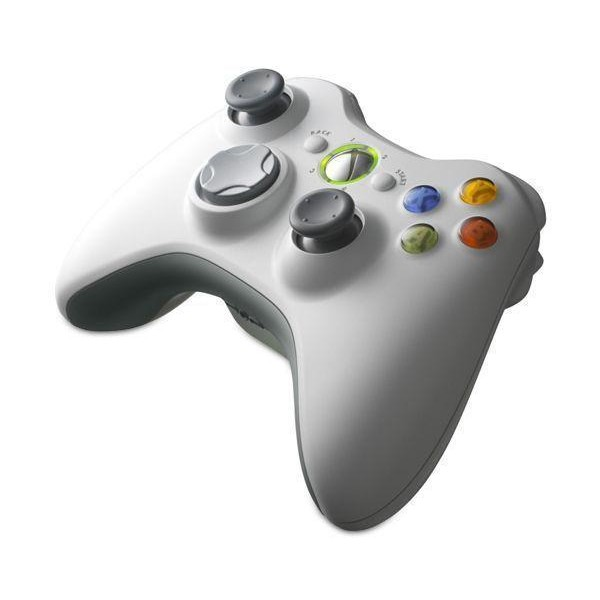
\includegraphics[width=13cm]{images/xbox360.jpg}
\end{center}      

\section{Exploring the terrain}
      \section{Adding Blocks}
        \subsection{Adding blocks with the second display system}
          You've already guessed it adding blocks with the second system was fairly easy (those functionalities weren't implemented with the first display system).\\
          Basically when adding a new block, we would ``refresh'' the surrounding blocks, in order to remove faces which were no longer visible.\\
          And adding to the scene the visible faces.

        \subsection{Adding blocks with the second display system}
          Even though this system boosted the Frames Per Seconds, it had it disadvantages and, adding blocks was one of them.\\
          When creating a material, once it has been displayed on the scene, other faces can't be added to it...\\ 
          Thus we had to think of something else. We came up with an intermediary solution : \\
          When the player wanted to add blocks, we would add faces (which were all distinct entities, just like the second display system) however, after a certain amount of blocks added, we would start a new thread and recreate another Material, when the new material would be done, we would swap it with the old one and destroy the old one!

      \section{Removing Blocks}
        Dealing with removing blocks with our third display system was really difficult. Mostly because we could not hide any part of the Manual object nor could we recreate it because it would have taken too much time.\\

        Fortunately, we discovered a way to edit manual objects but it involved using pointers. However at dedalus we like taking risks and, we decided to use pointers!\\
        Basically, all the points we add to a Manual object are stored in a Vertex buffer and, using pointers we can access them :

        \begin{lstlisting}
            vertexBuffer = this.manualObjectData.vertexData.vertexBufferBinding.GetBuffer(posEl.Source);
            vBufferList.Add(vertexBuffer);
            byte* pVertex = (byte*)vertexBuffer.Lock(HardwareBuffer.LockOptions.HBL_NORMAL) + vertexBuffer.VertexSize * this.mIndexInVertexBuffer[elemPosition];
            float* pReal;


            for(int i = 0; i < numFaces * 4; i++) {
                posEl.BaseVertexPointerToElement(pVertex, &pReal);

                pReal[0] = 0; pReal[1] = 0; pReal[2] = 0; //A vertex is a Vector3
                pVertex += vertexBuffer.VertexSize;
            }

            vertexBuffer.Unlock();
            \end{lstlisting}

            One of the annoying part is that vertexBuffer which is of type HardwareVertexBufferSharedPtr is an object which is created by Ogre and, when used will be automatically disposed by this one. However C \# has a garbage collector which will also try to dispose it after Ogre takes care of it. Thus when the garbage collector tries to dispose of the vertex buffer, the program crashes.\\


            Solving this bug was really complicated and, we couldn't find much help on the Mogre's forum.
\newpage

      \section{Inventory}
	 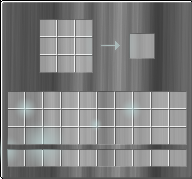
\includegraphics[width=6cm]{images/Inventory.png}

	 \begin{textblock}{0.45}(0.44,0.17)
    		Another big news for the oral presentation is the inventory. The system looks like much the minecraft one's. It's a drag and drop inventory.\\
Basically you can click on almost any cases and move to the desired case without releasing the click. On release, the items will swap. It may seems simple but it's much harder than it looks to implement.\\
The items can be stacked up to 64 on the same case. Then another case will be used if you want more ... 
         \end{textblock}
\bigskip\bigskip
The inventory is updated as soon as a block is added or deleted. Indeed the addition of a block means that a block must be taken from your inventory, the deletion entails an addition in the inventory. The bar on the bottom represent the select bar and the 10 cases on the top is the crafting table.

\section{Select bar}
	The select bar is always on the foreground at the bottom of the screen. It has a selector pointing on a specific case of the bar. It's really useful since it is the tool that allow the player to choose which block will be acting on the main action button.\\
Thus the selector determines whether the click will entails a shoot or a block addition and which texture will be used.\\

It's different from the inventory because it doesn't store anything. It's more like a pointer, pointing to the last bar of the inventory.
\begin{center}
 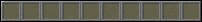
\includegraphics[width=6cm]{images/selectBar.png}
\end{center}
      \section{Crafting}
	The crafting table is opened at the same time than the inventory. As the name let you guess, it allows you to craft items from a predefined recipe. The ingredients go to the 9nth cases at the left, the result appears on the right case. \\
The recipe are quite interesting since they are stored as a general tree. Indeed it's not enough to place the right amount of item, they also have to be at the right place on table ! Even if they are only 3x3 cases, it makes lots of possibilities.
\newpage
	\section{Builder}
\bigskip
 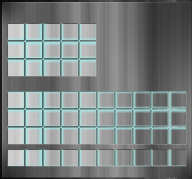
\includegraphics[width=7cm]{images/Builder.png}
\begin{textblock}{0.45}(0.5,0.17)
    		This GUI looks quite the same than the inventory. The 4 lines below have the same roles. But the 15 first cases are more interesting. This GUI is opened by a construction block (see below). The selection of the building is made on the right of the GUI. As soon as a building is selected we can drop the resources, and they will be added to the construction block's inventory. If we exit the GUI without giving enough resources, the building will be build with ghost blocks. It means the building won't be there (no collisions) but we can see what the building will looks like and where will it be exactly. The resources are definitely lost from the inventory.
         \end{textblock}

\begin{textblock}{0.33}(0.1,0.55)
	Else if all the needed resources have been given, the building will instantly be built. A problem we encountered id the position of the building relatively to the construction block.We don't want the building to build up on a character. The solution was to make the central symetrie relatively to the construction block if the player is in the initial building position. 
         \end{textblock}

\begin{textblock}{0.45}(0.48,0.5)
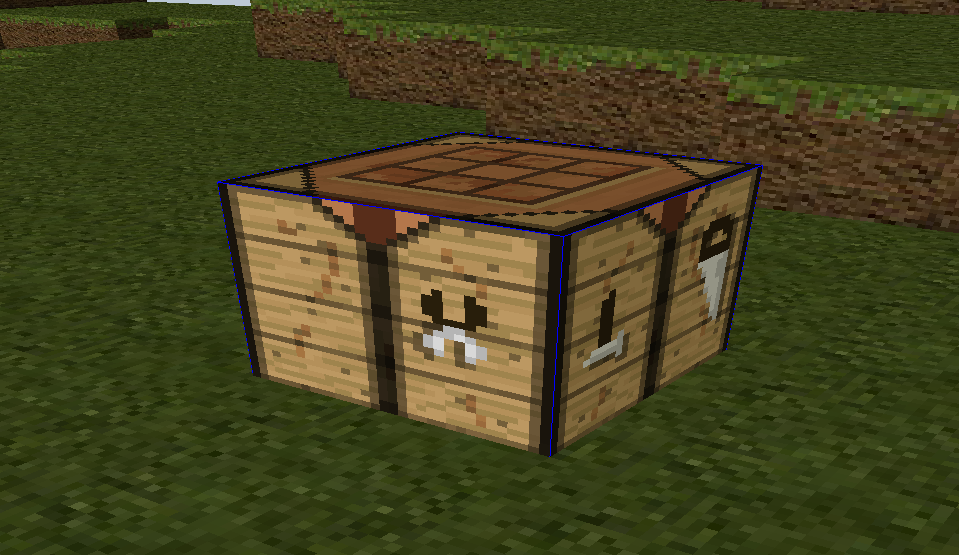
\includegraphics[width=10cm]{images/constructionBlock.png}
         \end{textblock}
	
    \chapter{\textcolor{blue}{Strategy}}
      
    Since our game is also a RTS game, it has a strategic part based on building a base and recruiting troops to help the player fight in his quest for defeating the evil. The RTS part is mainly made of building a base, recruit troops and kicking the enemy's butt.\\

      \section{Build your own Base}

 Like in every RTS game, the player can build his own base to produce resources or recruit troops. Building materials can be collected by the player as he travel through the map by mining or collected by NPCs in resource deposits build by the player. All the available buildings can be found on the ingame builder panel by placing a construction block then choosing the right one among the possible ones.\\

    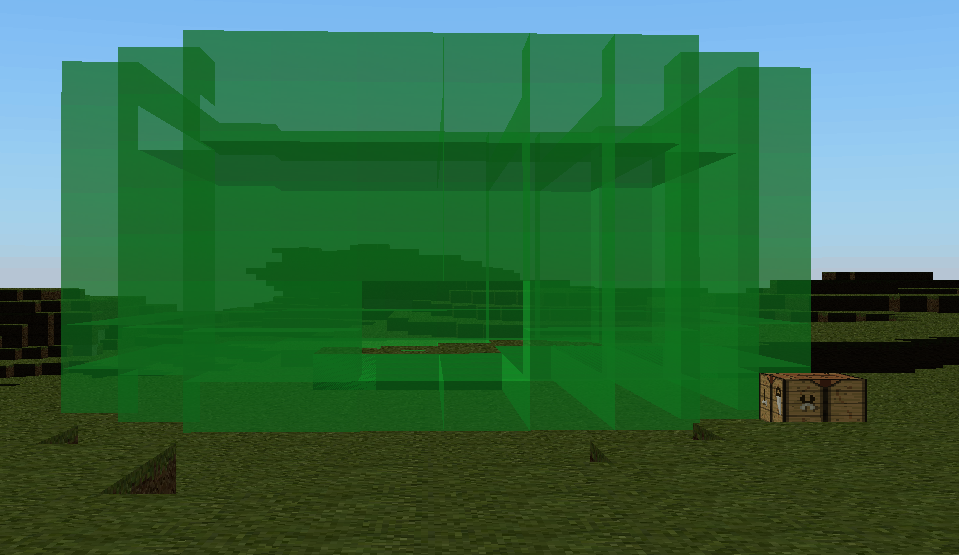
\includegraphics[width=15cm]{images/construction_block_ghost.png}

The selected building will appear as a ghostly green jelly while it is being built and will become clearer as the player place building material in the construction block linked to the structure. \\
 

      \section{Buy your army of Robots}


  ~\\
Once the main base has been built, the player can start recruiting robots in barracks to make them fight the evil robots in his stead. The robots will fight alongside with the player as he go further in defeating his foes to take over their base and the portal to go to the next stage. \\

    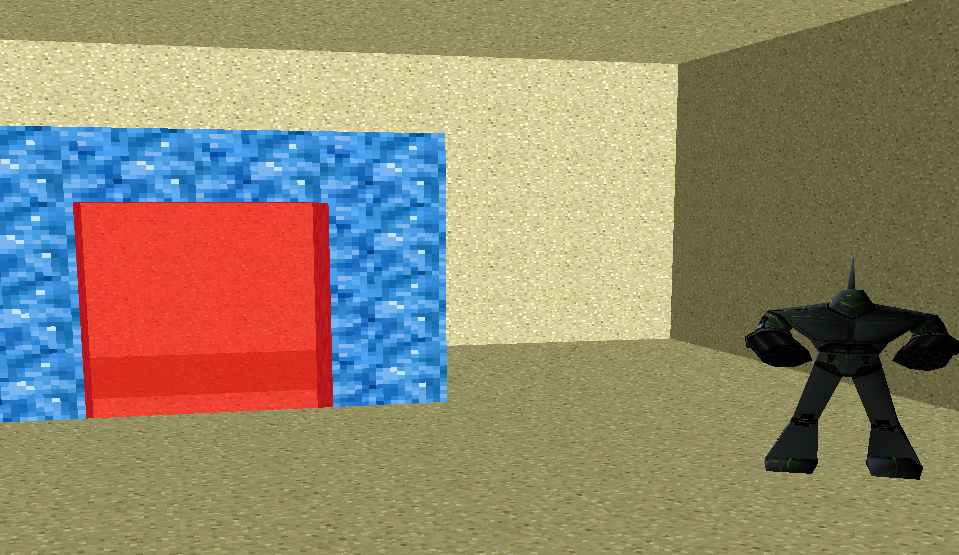
\includegraphics[width=15cm]{images/desert_screen.png}

When accessing to the next stage the player will keep all his collected resources. However, once the portal on a map is found, since the portal can only be used by the ``chosen one",the player will be the only one to get transported to the next map. Also will he have to make a new base each time he discovers a new island and recruit new troops. \\

      \section{Fight against foes}

    \begin{textblock}{0.4}(0.120,0.7)
   In order to win against his foes, the player will have to come up with new strategies to corner his enemies trap them and crush them and easily defeat them. The enemies are controlled by a simple AI corresponding to the only available level difficulty which is hard mode, because every game must have a hard mode because the normal mode is usually far to simple .\\

  The foe robots will keep shooting at the closest target until it is killed. Also would it be wise to put the troops in front of the player's character so that it can pass through the ambush or battle.\\
    \end{textblock}

    \begin{textblock}{0.6}(0.53,0.675)
    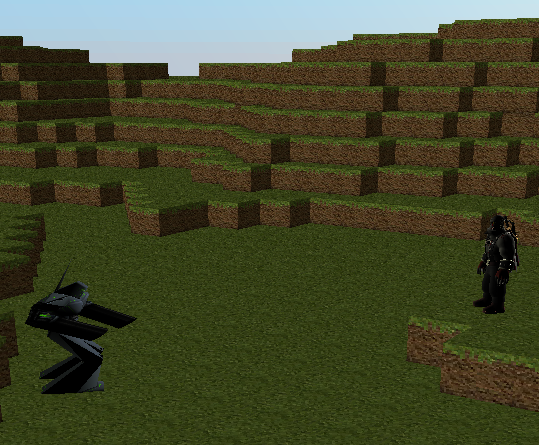
\includegraphics[width=9cm]{images/shoot.png}
    \end{textblock}


 \newpage

  The very special aspect of our game in a strategic way of speaking lays in the power the player has to alter the map. This ability can be used to built walls around the player's base or even the enemy's base, built mazes for the foes to get ``lost" in and get slowed down. The player can also built traps for the opponent to fell in by digging holes at specific placements since the robots aren't equipped with jet packs and therefore cannot climb back up whenever the fall into a hole. Bridges or tunnels can also be dig and built to allow the allied troops to access some hardly accessible places like a flying island or the other side of a huge natural wall. \\

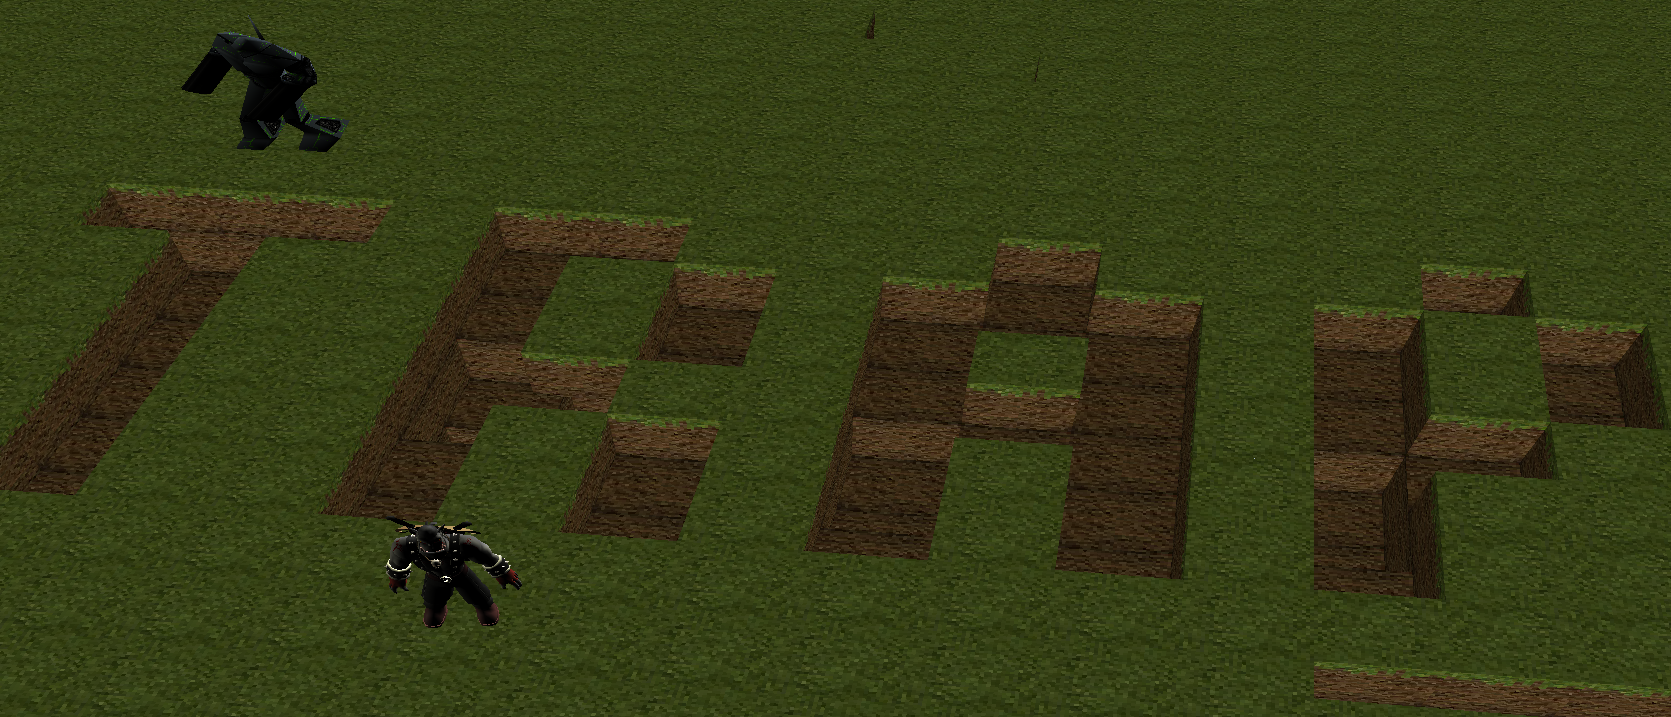
\includegraphics[width=15cm]{images/trap.png}



  Aside from the troops management aspect, some maps will not allow the player to display allied robots to help him fight. For example, while passing through the ``Snowy Mounts range" the player will not be able to rely on troop support since the landscape doesn't suit the robots at all. Also will he need to use his map alteration skill to the maximum in order to escape from his foes while looking for the portal leading to the next stage.\\

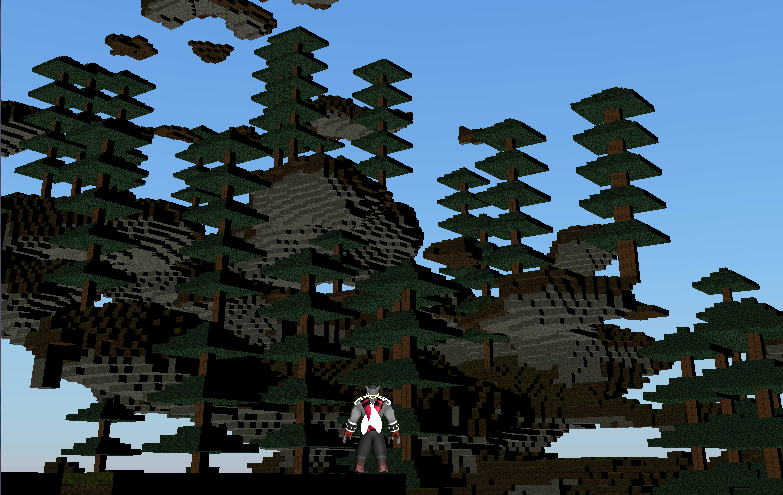
\includegraphics[width=18cm,height=10cm]{images/mountains_view.png}

      \section{PathFinding}
        Pathfinding refers to the plotting, by a computer application, of the shortest route between two points. At its core, a pathfinding algorithm searches a graph by starting at one vertex and exploring adjacent nodes until the destination node is reached. Although graph searching methods such as a breadth-first search would find a route if given enough time, other methods, which explore the graph, would tend to reach the destination sooner. \\
        It is useful when integrating an IA. With it, a character will dodge holes and dead ends. An example use of the pathfinding : if an enemy see the player, the algorithm will find the shortest path the enemy can take to come and attack the player.
        
        \subsection{A star 2d}
          The A* algorithm combines features of uniform-cost search and pure heuristic search to efficiently compute optimal solutions. A* algorithm is a best-first search algorithm in which the cost associated with a node is $ f (n) = g(n) + h(n) $ , where$  g(n) $  is the cost of the path from the initial state to node $ n $ and $ h(n) $ is the heuristic estimate or the cost or a path from node $ n $ to a goal. Thus, $ f(n) $ estimates the lowest total cost of any solution path going through node $ n $. At each point a node with lowest $ f $ value is chosen for expansion. Ties among nodes of equal $ f $ value should be broken in favor of nodes with lower $ h $ values. The algorithm terminates when a goal is chosen for expansion.

          A* algorithm guides an optimal path to a goal if the heuristic function $ h(n) $ is admissible, meaning it never overestimates actual cost.

          For Puzzle, A* algorithm, using these evaluation functions, can find optimal solutions to these problems. In addition, A* makes the most efficient use of the given heuristic function in the following sense: among all shortest-path algorithms using the given heuristic function $ h(n) $. A* algorithm expands the fewest number of nodes.

          The main drawback of A* algorithm and indeed of any best-first search is its memory requirement. Since at least the entire open list must be saved, A* algorithm is severely space-limited in practice, and is no more practical than best-first search algorithm on current machines. \\

\begin{center}
 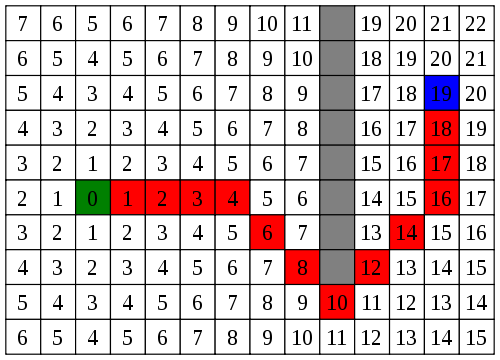
\includegraphics[width=12cm]{images/AStar_2.png}
\end{center}

        \subsection{A star 3d}
          Implementing the third dimensions for the A star algorithm was easier then expected. The A star in two dimensions uses an open list where it stores all the possible nodes which can be part of the best path. To find the best path, the algorithm look at all the adjacent nodes of each nodes in it's open list.\\

          To implement the third dimensions we only had to change the function which returns the adjacent nodes which only send the adjacent nodes on the same Y level we added two more levels and had to make sure the algorithm would not return a  path in the air.
  \begin{center}
    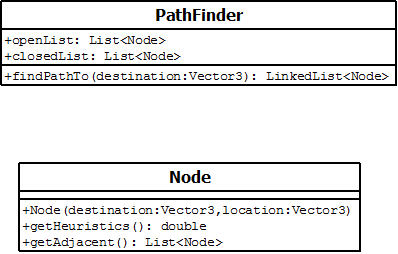
\includegraphics{images/Astar.png}
  \end{center} 

\subsection{Integration to our game}
	The A star 3d let us stores the desired path in a stack. But this isn't that simple to use it, we can't just translate the node to the next position and move on like this. Indeed we want our animations to be playable, it means that the AI must move forward and turn around to the right direction. Rotations and translations in a 3d world, it sounds like a painful idea ...\\

What we did is that we computed the needed yaw rotation for the AI. It then yaw continuously until it almost reaches the desired angle. As soon as the difference of rotation is little enough, we can begin to move forward the character. We didn't moved it before because we don't want him to move away nor to miss his target point. 

      \section{Global AI}
	What we call the global AI refers to the real opponent of the player. It's the AI that control the opposite faction, build buildings and create an army. It's only goal is to destroy the player. The difficulty here is to make an AI not to dumb, not to invincible. The easiest way to do that we think is to adapt the AI according to the player. \\

A weight is set for each action the player can do (placing a building, spawning a unit). The most important this action is, the heavier his weight will be. The weight represents a panel that the AI can do. Every 4xx milliseconds, the AI makes a choice and the heavier the weight is, the most important action the AI could do.\\

To choose the best action, the AI bases its choice on the player situation. Basically if the difference in any field (the capacity, the number of units, ...) is too high, the AI will try to re equilibrate this. There is also always a part of random in the choice of the AI.
  \begin{center}
    
\includegraphics[width=14cm]{images/hal.jpg}
  \end{center} 

    \chapter{\textcolor{blue}{Graphics}}
    To make our game look even more personal we decided to redesign all the menus and Sinbad's skin in a science fiction style. Apart from renewing our game's look, we also added special effects like using particles.\\
            \section{Menus skins}

At first we wanted to give our game a steam punk look but considering all the specific features of steam punk we decided it would take to long to draw all the gears, wavering screens, discarded places and industrial wastelands. Also we decided to go for a simple science fiction spaceship looking theme with blue lights and screens. \\

\includegraphics[width=15cm]{images/Skins/Load_Scenario_normal.png}

A total of eight menus were created or redesigned according to the chosen theme: Main Menu, Play Menu, Option Menu, Scenario Load Menu, In-game Menu, two Scenario Editor Menus and finally a Death Screen Menu. \\

\newpage

Each menu was though so that the player could easily understand how they work. When the mouse is over a interactive component it become highlighted in a yellowish light to show the player he can click. \\

\begin{textblock}{0.5}(0.125,0.140)
\includegraphics[width=7cm]{images/Skins/ingame_menu_normal.png}
\end{textblock}

\begin{textblock}{0.5}(0.5,0.140)
\includegraphics[width=7cm]{images/Skins/ingame_menu_back.png}
\end{textblock}


~\\~\\~\\~\\~\\~\\~\\~\\~\\~\\~\\~\\~\\~\\~\\~\\~\\

One can also notice the evolution of the shadows on each menu as the time passed by and therefore guess the order in which they were made, starting with the Main Menu to the in-game menu.\\
It shows the motivation of the team as the oral presentation is arriving faster and faster and the motivation of the graphist to make a better looking game than the groups in the next room. \\

\begin{textblock}{0.5}(0.120,0.5)

\includegraphics[width=8cm]{images/Menus/Menu_Normal_view.png}

\end{textblock}

\begin{textblock}{0.5}(0.5,0.5)

\includegraphics[width=8cm]{images/Menus/menu_play_normal.png}

\end{textblock}

\begin{textblock}{0.5}(0.120,0.7)

\includegraphics[width=8cm]{images/Menus/Menu_Options_normal.png}

\end{textblock}

\begin{textblock}{0.5}(0.5,0.7)

\includegraphics[width=8cm]{images/Menus/Load_Scenario_normal.png}

\end{textblock}

\newpage

      \section{Sinbad's skins}

Sinbad may be Mogre's mascot, we found him so stylish that we decided to keep him as the main character of SkyLands. However, since it is our game, we changed Sinbad's skin to make him look 20\% cooler and the game 100\% more personal. We modified the .tga files that define Sinbad's skin by using specific functions of Photoshop that enable the user to modulate the colors one by one.\\

\begin{textblock}{0.4}(0.1,0.25)

\includegraphics[width=7cm]{images/Skins/Neo_sinbad.png}

\end{textblock}
\begin{textblock}{0.4}(0.55,0.25)

\includegraphics[width=7cm]{images/Skins/Vamp_sinbad.png}

\end{textblock}


\begin{textblock}{0.4}(0.33,0.55)

\includegraphics[width=7cm]{images/Skins/normal_sinbad.png}

\end{textblock}

~\\~\\~\\~\\~\\~\\~\\~\\~\\~\\~\\~\\~\\~\\~\\~\\~\\~\\~\\~\\~\\~\\~\\~\\~\\~\\~\\~\\~\\~\\~\\~\\~\\~\\~\\~\\~\\~\\~\\~\\~\\~\\
Sinbad now possess two new skins 20\% cooler the the original one, a blue one from the Neo clan and a red one from the Vamp clan which are respectively the evil twisted minded soldiers from the villains empire and the chosen saviors of the universe meant to fight against evil for the freedom of the universe. \\

\newpage

      \section{Particles}

Still wanting to make our game 20\% cooler than Minecraft and Starcraft brought as one we had to had a particles engine. Ours is very simple, we use 2D images that are turned according to the location of the camera so that it can create an illusion of 3D. \\

The particles are use for example in the Snowy Mounts Range to represent snow. We also had mist on every map in order to reduct the player vision field and the FPS of the game but as we noticed that it didn't change anything, we eventually removed the mist, letting the player see as far as ground exists.\\


\includegraphics[width=16cm]{images/snowy_mounts_range.png}

~\\
 
In the Snowy Mounts Range, after it has stopped snowing, a small layer of snow still remains on the highest flying islands.\\
    \chapter{\textcolor{blue}{Scenario Editor}}
      \section{Basic Idea}
				The idea  of the scenario editar was to be able to add things such as particle, sound or spawn units when the player would enter a certain block.\\
				The basic gist of it is as follow : a scenario is a succession of structures.
      \section{Structures}
				Those structures are buildings whose height cannot go above 16 by 16 by 16 :\\
				
				\includegraphics[width=9cm, height=7cm]{images/Scenario.png}
				
      \section{Scripting}
    \chapter{\textcolor{blue}{Sound Engine}}
	We realized that there was something missing in our game, the sound. Sound is really important in a game, it is usely what gives the player emotions, it is what create the magie of certain scenes.
	So, to put sound in our game, we created a sound engine. This engine can play sounds depending on the situation, for example during intense situations, the music will be playing louder and faster. The sound level coming from noises made by monsters will also depend on the distance between him and the player.
	
		\begin{figure}[h]
				\includegraphics[width=9cm, height=7cm]{images/FLStudio/1.JPG}
				\includegraphics[width=9cm, height=7cm]{images/FLStudio/2.JPG}
				\begin{center}\it The sin(x) * cos(y) and the sinus 3d function\end{center}
			\end{figure}
	
    \chapter{\textcolor{blue}{Conclusion}}
    
\end{document}